\documentclass{article}

% if you need to pass options to natbib, use, e.g.:
\PassOptionsToPackage{numbers, compress}{natbib}
% before loading neurips_2026

% The authors should use one of these tracks.
% Before accepting by the NeurIPS conference, select one of the options below.
% 0. "default" for submission
\usepackage[dblblindworkshop]{neurips_2026}
% the "default" option is equal to the "main" option, which is used for the Main Track with double-blind reviewing.
% 1. "main" option is used for the Main Track
%  \usepackage[main]{neurips_2026}
% 2. "position" option is used for the Position Paper Track
%  \usepackage[position]{neurips_2026}
% 3. "eandd" option is used for the Evaluations & Datasets Track
 % \usepackage[eandd]{neurips_2026}
% 4. "creativeai" option is used for the Creative AI Track
%  \usepackage[creativeai]{neurips_2026}
% 5. "sglblindworkshop" option is used for the Workshop with single-blind reviewing
 % \usepackage[sglblindworkshop]{neurips_2026}
% 6. "dblblindworkshop" option is used for the Workshop with double-blind reviewing
%  \usepackage[dblblindworkshop]{neurips_2026}
% 7. "education" option is used for the Education Track
%  \usepackage[education]{neurips_2026}


% After being accepted, the authors should add "final" behind the track to compile a camera-ready version.
% 1. Main Track
 % \usepackage[main, final]{neurips_2026}
% 2. Position Paper Track
%  \usepackage[position, final]{neurips_2026}
% 3. Evaluations & Datasets Track
 % \usepackage[eandd, final]{neurips_2026}
% 4. Creative AI Track
%  \usepackage[creativeai, final]{neurips_2026}
% 5. Workshop with single-blind reviewing
%  \usepackage[sglblindworkshop, final]{neurips_2026}
% 6. Workshop with double-blind reviewing
%  \usepackage[dblblindworkshop, final]{neurips_2026}
% Note. For the workshop paper template, both \title{} and \workshoptitle{} are required, with the former indicating the paper title shown in the title and the latter indicating the workshop title displayed in the footnote.
% For workshops (5., 6.), the authors should add the name of the workshop, "\workshoptitle" command is used to set the workshop title.
% \workshoptitle{WORKSHOP TITLE}
% 7. Education Track
% \usepackage[education, final]{neurips_2026}

% "preprint" option is used for arXiv or other preprint submissions
 % \usepackage[preprint]{neurips_2026}

% to avoid loading the natbib package, add option nonatbib:
%    \usepackage[nonatbib]{neurips_2026}

\usepackage[utf8]{inputenc} % allow utf-8 input
\usepackage[T1]{fontenc}    % use 8-bit T1 fonts
\usepackage{hyperref}       % hyperlinks
\usepackage{url}            % simple URL typesetting
\usepackage{booktabs}       % professional-quality tables
\usepackage{amsfonts}       % blackboard math symbols
\usepackage{nicefrac}       % compact symbols for 1/2, etc.
\usepackage{microtype}      % microtypography
\usepackage{xcolor}         % colors
\usepackage{natbib}
\usepackage{tikz}
\usepackage{verbatim}
\usepackage{fancyvrb}
\usepackage{subcaption}
\usepackage{amssymb}
\usepackage{amsmath}
\usepackage{bbm}
\usepackage{enumitem}
\usetikzlibrary{arrows.meta,calc,positioning}

\setlength{\textfloatsep}{8pt plus 2pt minus 2pt}
\setlength{\floatsep}{8pt plus 2pt minus 2pt}
\setlength{\intextsep}{8pt plus 2pt minus 2pt}
\setlength{\abovecaptionskip}{4pt}
\setlength{\belowcaptionskip}{-2pt}
%\setlist[itemize]{leftmargin=*, topsep=2pt, itemsep=1pt, parsep=0pt}

\input{macros}

% Note. For the workshop paper template, both \title{} and \workshoptitle{} are required, with the former indicating the paper title shown in the title and the latter indicating the workshop title displayed in the footnote. 
% \workshoptitle{The First Workshop on Interpreting Agent Behavior - NeurIPS 2026}
\title{How Agents Know but Fail to Act:\\ Belief Action Gap in Language Model Agents}


% The \author macro works with any number of authors. There are two commands
% used to separate the names and addresses of multiple authors: \And and \AND.
%
% Using \And between authors leaves it to LaTeX to determine where to break the
% lines. Using \AND forces a line break at that point. So, if LaTeX puts 3 of 4
% authors names on the first line, and the last on the second line, try using
% \AND instead of \And before the third author name.


\author{%
  David S.~Hippocampus\thanks{Use footnote for providing further information
    about author (webpage, alternative address)---\emph{not} for acknowledging
    funding agencies.} \\
  Department of Computer Science\\
  Cranberry-Lemon University\\
  Pittsburgh, PA 15213 \\
  \texttt{hippo@cs.cranberry-lemon.edu} \\
  % examples of more authors
  % \And
  % Coauthor \\
  % Affiliation \\
  % Address \\
  % \texttt{email} \\
  % \AND
  % Coauthor \\
  % Affiliation \\
  % Address \\
  % \texttt{email} \\
  % \And
  % Coauthor \\
  % Affiliation \\
  % Address \\
  % \texttt{email} \\
  % \And
  % Coauthor \\
  % Affiliation \\
  % Address \\
  % \texttt{email} \\
}


\begin{document}


\maketitle


\begin{abstract}
Language model (LM) agents can fail due to a variety of reasons and distinguishing the failure mode is important because they require different explanations and interventions. We study how state beliefs, action values, and action preferences interact as LM agents reason and commit to decisions in text-rendered grid worlds. We estimate task-relevant beliefs using report-based and representation-based probes and action values using inverse reinforcement learning. We find that task-relevant state and value information is often represented more reliably than it is reflected in behaviour. Tracking action preferences throughout reasoning further shows that decisions sharpen around a commitment point, belief uncertainty decreases near commitment, and unsuccessful decisions tend to commit later, although individual belief changes do not consistently explain shifts in action preference. Finally, causal interventions show that actions strongly follow patched reasoning trajectories, whereas altering pre-reasoning state representations alone does not reliably change behaviour. Together, our results suggest that some agent failures arise not from missing task-relevant information, but from how available information is translated into and stabilized as an action. Our framework helps to distinguish between belief-related failures from failures of action selection and identify when represented information becomes causally relevant to behaviour.

\end{abstract}


\section{Introduction}

As language models are increasingly used as agents that observe, reason about, and act within external environments, evaluating their quality requires assessing whether they represent those environments accurately and how they translate representations into appropriate actions \cite{wang2024survey}. Evaluation based on outputs alone cannot answer these questions and therefore often cannot diagnose \emph{why} an agent fails. An incorrect action may result from an inaccurate belief about the current environment state, a failure to translate an accurate belief into an appropriate action, or a value function that assigns high value to states that are undesirable for the task.

These failure modes can produce similar observable behaviour despite having different underlying causes, and distinguishing among them is important, particularly from a safety perspective \cite{amodei2016concrete}. An agent that acts incorrectly because it misperceives its environment presents a fundamentally different failure mode from one that represents the environment accurately but nevertheless selects an incorrect or undesirable action. Without identifying whether a failure originates in the agent's beliefs, its assigned values, or the mechanism that translates them into actions, an intervention may correct the observed behaviour without addressing its underlying cause.

To analyse these failure modes, we view an agent's behaviour as the result of three interacting components. The first is its belief about the current state of the environment, where we use \emph{belief} to refer to any interpretable internal representation of the environment given the information available to the agent. The second is its value or preference structure, which determines how it ranks possible states, actions, or trajectories. The third is its decision mechanism, which defines how beliefs and values are converted into a selected action. Distinguishing these components supports a more precise diagnosis of whether a failure arises from inaccurate state information, inappropriate preferences, or the mechanism through which available information influences behaviour.

Existing work provides complementary methods for studying these components. White-box methods test whether model activations encode spatial structure and other task-relevant beliefs \cite{li2022emergent,nanda2023emergent,gurnee2024language,arghal2026behavioural}, while behavioural approaches infer latent values or preferences from observed decisions, including through inverse reinforcement learning \cite{ziebart2008maximum,holgado2026learning} and recent analyses of preferences expressed by language-model agents \cite{khan2026agents,lu2025aligning}. Other work shows that information about future responses can be decoded before those responses are produced \cite{belrose2023eliciting,pal2023future,dong2025emergent}, while chain-of-thought traces provide an additional view of decision formation but need not faithfully reflect the computations responsible for the final answer \cite{turpin2023language,lanham2023measuring,gao2024aligning}. Recent work has also begun to connect state understanding, expressed values, reasoning, and actions within a common behavioural framework \cite{leng2026suva}.

Together, these approaches provide complementary views of agent decision-making, but they do not by themselves identify where the transition from represented information to behaviour fails. Decodable state information need not be used in action selection, an observed preference does not reveal whether it follows from an incorrect state estimate or an inappropriate valuation, and a reasoning trace may correlate with a decision without causally determining it. We therefore analyse state representation, inferred preference, action formation, and causal influence within the same decision process. This lets us ask whether task-relevant information is missing, whether the available representation supports the wrong action, or whether information that supports an appropriate action nevertheless fails to govern the model's choice.

We investigate these questions in a text-rendered grid world, where the possible states and actions can be enumerated and the transition dynamics and optimal policy are known. We estimate task-relevant beliefs from internal model activations and explicit reports, infer value structure from representations and behaviour using inverse reinforcement learning, track how beliefs and action preferences evolve during reasoning, and apply causal interventions to test when represented information begins to determine the final action.

Our main contributions are as follows:
\begin{itemize}[
leftmargin=1.4em,
label=\raisebox{0.35ex}{\rule{0.75ex}{0.75ex}},
labelsep=0.5em
]
\item \textbf{Belief--action diagnostic analysis.}
We distinguish failures caused by inaccurate state beliefs from cases in which task-relevant information is represented but does not lead to the appropriate action.

\item \textbf{Temporal analysis of decision formation.}
We track beliefs and action preferences throughout reasoning and identify when the final action becomes stable.

\item \textbf{Causal tracing of decision formation.}
We intervene on reasoning trajectories and internal model activations to determine when represented information causally affects behaviour rather than being merely decodable.

\item \textbf{Empirical evidence of the belief--action gap.}
We find that task-relevant information is represented more reliably than it is expressed in behaviour, showing that failures can arise in the mechanism that converts represented state information into action.
\end{itemize}



\section{Estimating Beliefs and Values}
\label{sec:estimating}

We characterise each agent decision using an estimated belief distribution $\hat q_t(s)$ over the current environment state, a fixed transition function $T$, a learned state-value function $g_\theta(s)$ that assigns a scalar value to each state, and the emitted action $a_t$. 
For diagnostic purposes, without assuming that the language model performs this computation internally, we define the utility of each action from the model's subjective perspective as the expected value of its successor state under the estimated belief distribution, given the transition function:
\begin{align}
    U_{\theta,t}(a)
    &=
    \mathbb{E}_{s \sim \hat q_t}
    \left[g_\theta\bigl(T(s,a)\bigr)\right].
    \label{eq:expected-action-preference}
\end{align}
We estimate $\hat q_t$ from model verbal reports and internal activations (\Cref{sec:estimating-beliefs}) and infer $g_\theta$ from state--action pairs using inverse reinforcement learning (\Cref{sec:estimating-values}). 
We then compare the expected successor-state value of the emitted action with the highest value assigned to any available action. 
The difference between these quantities is the regret of $a_t$, which we use to define the \emph{belief--action gap}. \todo{ND: consider actually putting an equation here for the gap?}


% Our initial goal is to determine whether there is a difference between the internal encodings of an agent i.e. beliefs and the actions it took. Finding this requires an estimate of what state the model takes itself to be in, an estimate of which states are preferable under the task, and the action the model ultimately selects. This section defines these quantities and shows how they are combined into the belief action gap.

\subsection{Grid World Environment}
\label{sec:env-data}

We study a language model agent in a fully observable, text-rendered grid world, following the setup of \citet{arghal2026behavioural}. 
The grid contains walls, open cells, a goal cell, a locked door that blocks the route to the goal, and a key that the agent must collect before passing through the door. 
The key is collected automatically when the agent enters its cell, after which the door becomes traversable. Transitions are deterministic: a valid movement changes the agent's position by one cell, whereas an action directed towards a wall or locked door leaves the agent in its current position.
Figure~\ref{fig:environment} shows an example grid.


\begin{figure}[htbp]
\centering

\begin{subfigure}[c]{0.42\textwidth}
\centering
\begin{BVerbatim}
  0 1 2 3 4 5 6 7 8
0 # # # # # # # # #
1 # . . . # . . . #
2 # . . . D . . . #
3 # . . . # . G . #
4 # . # # # # # # #
5 # . . . . . . . #
6 # . . . # . K . #
7 # . . A # . . . #
8 # # # # # # # # #
\end{BVerbatim}

\caption{}
\label{fig:grid_text}
\end{subfigure}
\hspace{0.02\textwidth}
\begin{subfigure}[c]{0.42\textwidth}
\centering
\includegraphics[width=0.6\linewidth]{figures/keydoorenv.png}
\caption{}

\label{fig:grid_visual}
\end{subfigure}

\caption{
Example DoorKey environment shown in text and spatial form.
The language model receives the text-rendered grid in \textbf{(a)}, while \textbf{(b)} visualises the same underlying environment used to define states, transitions, and planner-optimal actions.
$A$ denotes the agent, $K$ the key, $D$ the door, $G$ the goal, and filled cells denote walls. \td{Can we use the same renderings as in the goal-directedness paper?}
}
\label{fig:environment}
\end{figure}

For a fixed grid layout $G$, we represent the environment state at decision step $t$ as
\begin{align}
    s_t
    &=
    (x_t,y_t,h_t,d_t),
    \label{eq:task-state}
\end{align}
where $(x_t,y_t)$ are the agent's grid coordinates, $h_t \in \{0,1\}$ indicates whether it is carrying the key, and $d_t \in \{0,1\}$ indicates whether the door is open. 
The layout $G$ specifies the fixed locations of walls, the key, the door, and the goal.
For our analyses, we use a fixed $9\times9$ grid layout. 
The grid contains 39 walkable cells and admits 117 valid task states after accounting for the three reachable key and door phases.

At each step, the language model agent receives the complete current grid, including coordinate labels, and its key possession status, but no previous environment states or actions.\todo{mention it is markovian?} It produces a sequence of reasoning tokens $R_t =(r_{t,1},\ldots,r_{t,m_t})$ and emits one action from $\mathcal A = \{\textsc{left},\textsc{right},\textsc{up},\textsc{down}\}$. 


Given $G$, a state $s$, and an action $a$, the known transition function $T_G(s,a)$ returns the successor state.
We use A$^{\star}$ search on the augmented state space in Equation~\ref{eq:task-state} (i.e., accounting for whether the key has been collected and whether the door has been opened) to compute the length $D_G^*(s)$ of a shortest valid path from $s$ to the goal \cite{hart1968formal}. 
The set of optimal actions is
\begin{align}
    A_G^*(s)
    &=
    \underset{a \in \mathcal{A}}{\operatorname{argmin}}\;
    D_G^*\bigl(T_G(s,a)\bigr),
    \label{eq:optimal-action-set}
\end{align}
which contains every action whose successor state lies on a shortest valid path to the goal.

\subsection{Estimating Beliefs}
\label{sec:estimating-beliefs}

We estimate the model's beliefs about task-relevant state variables using two approaches. 
Representation-based estimation decodes state variables from the model's activations, whereas report-based estimation measures what the model asserts when directly queried about the environment.
The two approaches currently overlap on a subset of state features, most directly local wall information. \mg{Why don't we cover the all state features with both approaches?}  
For these shared features, we compare their predictions at the same environment decision step $t$ to measure agreement between explicitly reported and internally decoded information. 
To compute the belief--action gap, we use the representation-based estimates; report-based estimates are analysed separately to test whether the model's actions are consistent with the state information it explicitly reports.


\subsubsection{Representation-based Belief Estimation}
\label{sec:activation-based-estimation}

We obtain representation-based belief estimates by training linear probes on language model activations to predict the components of the task-relevant state \cite{alain2016understanding,gurnee2024language}. 
Let $p$ denote a contiguous region of the token sequence preceding the model's action, located either in the prompt or in the reasoning trace. 
For decision step $t$ and model layer $\ell$, let $\mathbf{u}_{t}^{(\ell,p)}$ denote the vector formed by concatenating the layer-$\ell$ activations at all token positions within $p$, in sequence order.

We train one probe for each state component in \Cref{eq:task-state}. 
Coordinates are decoded jointly as a single categorical variable over grid locations, $z_{\mathrm{pos}}=(x,y)$. 
The other targets are key possession $z_{\mathrm{key}}=h$ and door status $z_{\mathrm{door}}=d$. 
Let $\mathcal Z_j$ denote the set of possible values for component $j$. The corresponding probe produces the distribution
\begin{align}
    q_{t,p,j}^{\mathrm{probe}}(z_j)
    &=
    \operatorname{softmax}
    \left(
        W_j \mathbf{u}_{t}^{(\ell,p)} + \mathbf{b}_j
    \right)_{z_j},
    \qquad z_j \in \mathcal Z_j.
    \label{eq:component-probe}
\end{align}
The probes are trained independently because their target variables have different domains and label spaces.

We combine the three component distributions into a distribution over complete task states.
Let $\mathcal S_G$ denote the set of valid states for layout $G$.
For a state $s=(x,y,h,d)$, we first form the factorised distribution
\begin{align}
    \widetilde q_{t,p}(s)
    &=
    q_{t,p,\mathrm{pos}}^{\mathrm{probe}}(x,y) \ 
    q_{t,p,\mathrm{key}}^{\mathrm{probe}}(h) \ 
    q_{t,p,\mathrm{door}}^{\mathrm{probe}}(d),
    \label{eq:factorised-probe-belief}
\end{align}
treating the three state components as conditionally independent given the model activation. 
We then normalise the distribution over valid states:
\begin{align}
    q^{\mathrm{probe}}_{t,p}(s)
    &=
    \frac{
        \mathbbm{1}[s \in \mathcal S_G]\,\widetilde q_{t,p}(s)
    }{
        \sum_{s' \in \mathcal S_G} \widetilde q_{t,p}(s')
    }.
    \label{eq:joint-probe-belief}
\end{align}
We quantify uncertainty in the resulting state estimate using Shannon entropy.
This allows us to distinguish incorrect but uncertain beliefs from incorrect beliefs held with high confidence and, when applied at multiple reasoning steps, to track changes in uncertainty over the course of reasoning.

We note that successful decoding establishes that information about a state variable is available in the model's activations, but it does not establish that the information influences the selected action \cite{elazar2021amnesic,belinkov2022probing}.
This distinction between decodability and causal use motivates the interventions in Section~\ref{sec:causal}.


\subsubsection{Report-based Belief Estimation}
\label{sec:report-based-estimation}

We further obtain report-based belief estimates by directly querying the language model about task-relevant features of the current state of the environment. 
The queries use the same rendered state supplied to the agent (cf.~\Cref{sec:env-data}).\mg{This used to say history-free, but if that's how the state is rendered to the agent, we should write that at the end of 2.1.} 
% A report elicited at reasoning position $p$ is conditioned on the prefix $R_{t,\leq p}=(r_{t,1},\ldots,r_{t,p})$; the prefix is empty when $p=0$.
For each state $s_t$ and immediately after a selected token region of interest $p$, we ask the model (i) whether the cell immediately to its left, right, above, and below is a wall; (ii) whether it is carrying the key; (iii) whether the door is open; (iv) whether the goal, key, or door is immediately adjacent in each cardinal direction; (v) the current coordinates of the agent, goal, key, and a door; and (vi) the immediate consequence of moving in each of the four candidate directions---in particular, whether the agent would hit a wall, obtain the key, or pass through an open door, as well as the coordinates of the successor state.
% Individual analyses use prespecified subsets rather than asking all questions at every $p$.
% The reasoning-time panel contains the six current-state categorical questions in (i)--(iii) and the three action-consequence questions for the action read out at that position; no scaled coordinate queries. \td{Verify that the list exactly matches every report-based question used in the experiments. Add section to the appendix with prompts, answer categories, and any relevant details (e.g., how answers are porcessed into answer categories)} \tx{I updated the list to reflect the query object as in my branch in repo reveng (origin/feat/counterfactual-patching); I added protocols as in Appendix \Cref{app:report-protocol}}
\Cref{app:report-protocol} gives the exact prompt templates, answer categories, and parsing rules. %, and panels.

For a categorical query, let $j$ index the queried variable and let $\mathcal Z_j=\{\texttt{yes},\texttt{no},\texttt{unknown}\}$ be its semantic answer set.
Free-text responses that do not parse are recorded separately as \texttt{invalid}; for sample-based runs we therefore take $\widetilde{\mathcal Z}_j=\mathcal Z_j\cup\{\texttt{invalid}\}$, while direct candidate-score runs use $\widetilde{\mathcal Z}_j=\mathcal Z_j$.
At decision step $t$ and region $p$, we construct a non-negative response score $w_{t,p,j}(z)$ for each $z\in\widetilde{\mathcal Z}_j$, either from candidate scores or from repeated samples:
\begin{align}
    w_{t,p,j}(z)
    &=
    \begin{cases}
        \exp\bigl(\ell_{t,p,j}(z)\bigr),
        & \text{when candidate scores $\ell_{t,p,j}(z)$ are available},\\
        \displaystyle \frac{1}{N}
        \sum_{n=1}^{N}
        \mathbbm{1}\!\left[z_{t,p,j}^{(n)}=z\right],
        & \text{when the response $z_{t,p,j}$ is sampled $N$ times},
    \end{cases}
    \label{eq:report-score}\\
\end{align}
Here $\ell$ is the temperature-scaled candidate logit, or the returned candidate log-probability, up to a common additive constant.
We then normalise these scores to obtain a distribution over $\widetilde{\mathcal Z}_j$:
\begin{align}
    q_{t,p,j}^{\mathrm{report}}(z)
    &=
    \frac{w_{t,p,j}(z)}
    {\sum_{z' \in \widetilde{\mathcal Z}_j} w_{t,p,j}(z')}.
    \label{eq:report-belief}
\end{align}
For logit-based scores, this is equivalent to the softmax transformation.
For sample-based scores, $q_{t,p,j}^{\mathrm{report}}$ is the empirical answer distribution.

% For each queried variable, we measure uncertainty using entropy,
% \begin{align}
%     H\!\left(q_{t,j}^{\mathrm{report}}\right)
%     &=
%     -\sum_{z \in \mathcal Z_j}
%     q_{t,j}^{\mathrm{report}}(z)
%     \log q_{t,j}^{\mathrm{report}}(z).
%     \label{eq:report-entropy}
% \end{align}
We evaluate the accuracy of report-based beliefs using the answer with the highest probability and use Shannon entropy to measure uncertainty.
% This allows us to distinguish incorrect but uncertain reports from confident incorrect beliefs, and when used at multiple steps through reasoning, it lets us follow changes in uncertainty throughout reasoning.
We also compare individual reports directly with the emitted action.
For example, reporting either that the cell to the left is a wall or that moving left would hit a wall, and then selecting \textsc{left}, constitutes a direct belief--action contradiction.
However, because these reports are elicited in separate forward passes and may reveal information that was not used during the original decision, we do not use them in the belief--action gap analysis.



\subsection{Estimating Values}
\label{sec:estimating-values}

Having estimated the model's beliefs, we use inverse reinforcement learning to infer state preferences from state--action pairs.
For a fixed grid layout $G$, let $g:\mathcal S_G\rightarrow\mathbb R$ denote a state-value function, where higher values indicate more preferred states.
We estimate this function using a one-step maximum-entropy IRL model \cite{ng2000algorithms,ziebart2008maximum}.


We represent each environment state $s$ by an activation-derived feature vector $\boldsymbol{\phi}_p(s)\in\mathbb R^d$.
Let $\mathcal I(s)=\{t:s_t=s\}$ denote the decision steps at which $s$ occurs in the dataset. For the fixed-grid IRL dataset, the environment has 117 valid states in total.
The 100 collected trajectories provide 1{,}822 state occurrences covering
54 distinct states (46\% of the state space); the remaining states are not
visited by the agent and therefore receive no feature vector. Occurrences are grouped by state when constructing $\boldsymbol{\phi}_p(s)$, so each of the 54 covered states is represented by the mean of its occurrences. \td{Report the number of distinct states and state occurrences used to construct these representations, either here or in the results section.}
For a token region of interest $p$ and model layer $\ell$, we average the activation vectors from these occurrences to obtain a state representation:
\begin{align}
    \boldsymbol{\phi}_p(s)
    &=
    \frac{1}{|\mathcal I(s)|}
    \sum_{t\in\mathcal I(s)}
    \mathbf{u}_t^{(\ell,p)}
    \in\mathbb R^d.
    \label{eq:activation-state-representation}
\end{align}
\td{Specify the model layer $\ell$ used to construct the state representations, either here or ideally in the analysis/results section directly}
Unless stated otherwise, all state representations use layers $\ell=7,15,23$, which
prior work found most informative for spatial state variables in this
environment \citep{arghal2026behavioural}. Each $\mathbf{u}_t^{(\ell,p)}$
concatenates the activations of three adjacent tokens in region $p$, giving
$d = 8640$. We consider the pre-reasoning prompt suffix and the post-reasoning output token positions.
We construct and standardise the representations separately and fit a separate value model for each region $p$.
The parameterised value model maps activation-derived feature vectors to scalar values, $g_\theta:\mathbb R^d\rightarrow\mathbb R$.
We use a linear parameterisation for this model,
\begin{align}
    g_\theta\bigl(\boldsymbol{\phi}(s)\bigr)
    &=
    \theta^\top\boldsymbol{\phi}(s).
    \label{eq:linear-state-value}
\end{align}

Because the transitions are deterministic and known, each candidate action $a$ has an exact successor state $T_G(s,a)$, so the action can be evaluated through the value $g_\theta(\boldsymbol{\phi}(T_G(s,a)))$ assigned to this successor.
We model action selection probability as
\begin{align}
    p_\theta(a\mid s,G)
    &=
    \frac{
        \exp\!\left(
            \beta g_\theta\bigl(\boldsymbol{\phi}(T_G(s,a))\bigr)
        \right)
    }{
        \sum_{a'\in\mathcal A}
        \exp\!\left(
            \beta g_\theta\bigl(\boldsymbol{\phi}(T_G(s,a'))\bigr)
        \right)
    },
    \label{eq:irl-policy}
\end{align}


where the fixed inverse-temperature parameter $\beta>0$ controls the sharpness of the induced policy.
Equation~\ref{eq:irl-policy} defines a Boltzmann choice model in which actions leading to more highly valued successor states receive higher probability.
Not every candidate successor state $T_G(s,a)$ is guaranteed to have an
activation-derived representation, since the trajectory dataset does not
necessarily visit every valid environment state. When constructing the IRL training set, we therefore retain a state--action observation only if
$\boldsymbol{\phi}(T_G(s,a'))$ is available for all four candidate actions
$a' \in \mathcal A$. If any successor state is absent from the state
representation table, the corresponding observation is excluded from the
IRL objective. Thus, the value model is trained only on source states for
which the complete one-step action comparison is defined.

\td{Clarify whether every candidate successor state occurs in the dataset. If not, explain how $\boldsymbol{\phi}(T_G(s,a))$ is defined when no activation is observed for that state.}

We call this model one-step IRL because it evaluates each action only through its immediate successor state and does not explicitly roll out future trajectories.
The state-value function may nevertheless encode longer-term desirability, because a successor can receive high value when it lies on a favourable future path. 
The assumption is that any such information is summarised by $g_\theta(\boldsymbol{\phi}(T_G(s,a)))$. 
This restriction allows the preference function to be estimated from local state--action comparisons. 

To fit the value models, we construct two datasets of state--action pairs.
The agent-supervised dataset $\mathcal D^{\mathrm{LM}}$ pairs each state
$s_t$ with the action $a_t$ emitted by the LM agent. For the
planner-supervised dataset $\mathcal D^{*}$, the planner first computes the
set of shortest-path optimal actions $A_G^{*}(s_t)$. When this set contains
multiple actions, one optimal action is selected as the training target
according to the planner's tie-breaking rule. We denote this target by
$a_t^{*}\in A_G^{*}(s_t)$. For evaluation, we additionally report whether the model's preferred action
belongs to the full optimal set $A_G^{*}(s_t)$, so predictions are not
penalised solely for selecting a different tied-optimal action. \td{Only one, or all optimal actions?}
For either dataset $\mathcal D$, we fit $g_\theta$ by minimising the negative log-likelihood of the corresponding action labels,\begin{align}
    \mathcal L(\theta)
    &=
    -\sum_{(G,s,a)\in\mathcal D}
    \log p_\theta(a\mid s,G).
    \label{eq:irl-objective}
\end{align}
The two value models therefore use the same state representations, model class, and optimisation procedure, but different supervision signals.
The agent-supervised model, $g_\theta^{\mathrm{LM}}$, estimates the state preferences most consistent with the LM agent's realised behaviour under the one-step choice model.
We interpret $g_\theta^{\mathrm{LM}}(\boldsymbol{\phi}(s))$ as an estimate of the agent's subjective value for state $s$.
The corresponding planner-supervised model is denoted by $g_\theta^{*}$.
Stronger held-out performance for $g_\theta^{*}$ than for $g_\theta^{\mathrm{LM}}$ would indicate that task-optimal action preferences are more reliably recoverable from the representations than the agent's realised action policy under this model class.
This would suggest that the representations contain task-optimal action information that is not consistently expressed in the agent's behaviour.
% The corresponding results are presented in Section~\ref{sec:value-results}.

\subsection{Quantifying the Belief--Action Gap}
\label{sec:belief-action-gap}

Having estimated beliefs and state values, we combine them to measure whether the emitted action is consistent with the preferences inferred from the agent's behaviour, under its uncertainty about the current environment state.

For a known state $s$, we define the regret of action $a$ under the agent-supervised value function $g_\theta^{\mathrm{LM}}$ as\looseness-1
\begin{align}
    \rho_\theta^{\mathrm{LM}}(s,a)
    &=
    \max_{a' \in \mathcal A}
    g_\theta^{\mathrm{LM}}\!\left(T_G(s,a')\right)
    -
    g_\theta^{\mathrm{LM}}\!\left(T_G(s,a)\right).
    \label{eq:state-action-regret}
\end{align}
This measures the value lost by taking action $a$ rather than the most highly valued available action.
It is zero when $a$ leads to a successor state with maximal value under the agent-supervised model and positive when an available alternative leads to a more highly valued successor.

Because the model is uncertain about the current state, we take the expectation of this regret under the representation-based belief distribution $q_{t,p}^{\mathrm{probe}}$.
For the action $a_t$ emitted at decision step $t$, we define the \emph{belief--action gap} as
\begin{align}
    \Delta_{t,p}^{\mathrm{LM}}
    &=
    \mathbb{E}_{s \sim q_{t,p}^{\mathrm{probe}}}
    \left[
        \rho_\theta^{\mathrm{LM}}(s,a_t)
    \right] =
    \sum_{s \in \mathcal S_G}
    q_{t,p}^{\mathrm{probe}}(s)
    \rho_\theta^{\mathrm{LM}}(s,a_t).
    \label{eq:belief-action-gap}
\end{align}
% We evaluate $\Delta_{t,p}^{\mathrm{LM}}$ at $p=0$, immediately before reasoning begins, and at $p=m_t$, after the final reasoning token and immediately before the action is generated.
A small gap indicates that the emitted action is consistent with the agent's inferred subjective preferences, given its uncertainty about the current state.
A large gap indicates that the agent-supervised model assigns higher value to the successors of other available actions.

This formulation distinguishes several possible sources of failure.
If an action is suboptimal under the true environment state but has a small belief--action gap, inaccurate state information provides a plausible explanation. 
If the decoded belief is accurate and the gap remains large, the failure lies downstream of state estimation. 
Comparing the action preferences induced by $g_\theta^{\mathrm{LM}}$ and $g_\theta^{*}$, then helps distinguish whether this inconsistency is better explained by the preference structure inferred from the agent's behaviour or by the mechanism that translates preferences into the emitted action.

\Cref{fig:environment} and \Cref{fig:belief_action_pipeline} summarise the environment and operational decomposition.
% \td{Revise figure (e.g., $a_t$ should connect to $g_{\theta}$) and fix caption.
% Also, split the grid example into another figure which also includes the visualisation of the 2d grid.}
% \begin{figure}[htbp]
% \centering
% \begin{tikzpicture}[
%     node distance=0.45cm and 0.6cm,
%     every node/.style={font=\footnotesize,align=center},
%     box/.style={
%         rounded corners,
%         draw=black,
%         thick,
%         minimum height=0.72cm,
%         minimum width=1.65cm,
%         inner sep=2pt
%     },
%     arrow/.style={-{Stealth[length=1.5mm]},thick}
% ]
% \node[box] (beh) {Behavioral\\belief};
% \node[box,above=1.5cm of beh] (rep) {Representational\\belief $\hat{q}$};

% \node[box,right=0.75cm of $(rep)!0.5!(beh)$] (cost) {One-step\\value $g_\theta$};
% \node[box,right=0.75cm of cost] (value) {Regret of action\\$\rho_\theta(s,a)$};
% \node[box,above right=0.15cm and 0.25cm of value] (act) {Taken\\action $a_t$};
% \node[box,below right=0.15cm and 0.15cm of value] (gap) {Belief--action\\gap $\Delta_t$};

% \draw[arrow] (rep.east) -- (value.west);
% \draw[arrow,dashed] (beh.east) -- (value.west);
% \draw[arrow] (cost) -- (value);
% \draw[arrow] (value) -- (act.west);
% \draw[arrow] (value) -- (gap.west);
% \draw[arrow] (act.south) -- (gap.north);
% \end{tikzpicture}
% \caption{Belief--action gap decomposition.}
% \label{fig:pipeline_panel}
% \end{figure}

\begin{figure}[t]
\centering
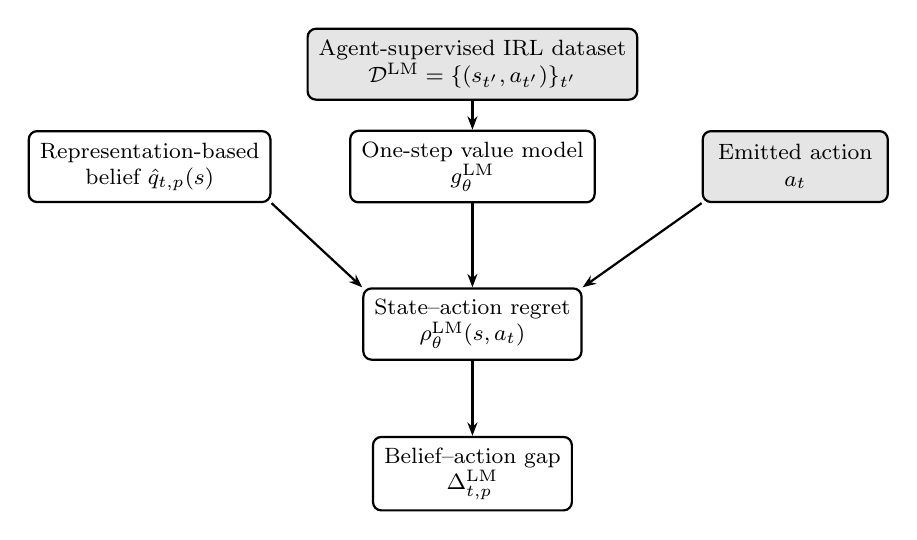
\begin{tikzpicture}[
    every node/.style={font=\footnotesize,align=center},
    box/.style={
        rounded corners=3pt,
        draw=black,
        thick,
        minimum height=0.9cm,
        minimum width=2.35cm,
        inner sep=4pt
    },
    observable/.style={
        box,
        fill=black!10
    },
    arrow/.style={-{Stealth[length=1.7mm]},thick}
]

% Observed IRL data
\node[observable, minimum width=3.0cm] (data) at (4.1,1.3)
{Agent-supervised IRL dataset\\
$\mathcal D^{\mathrm{LM}}=\{(s_{t'},a_{t'})\}_{t'}$};

% Main quantities
\node[box] (belief) at (0,0)
{Representation-based\\belief $\hat q_{t,p}(s)$};

\node[box] (value) at (4.1,0)
{One-step value model\\$g_\theta^{\mathrm{LM}}$};

\node[observable] (action) at (8.2,0)
{Emitted action\\$a_t$};

\node[box] (regret) at (4.1,-2.0)
{State--action regret\\$\rho_\theta^{\mathrm{LM}}(s,a_t)$};

\node[box] (gap) at (4.1,-3.9)
{Belief--action gap\\$\Delta_{t,p}^{\mathrm{LM}}$};

% Relations
\draw[arrow] (data.south) -- (value.north);
\draw[arrow] (belief.south east) -- (regret.north west);
\draw[arrow] (value.south) -- (regret.north);
\draw[arrow] (action.south west) -- (regret.north east);
\draw[arrow] (regret.south) -- (gap.north);

\end{tikzpicture}
\caption{
Operational decomposition of the belief--action gap.
Grey boxes denote observed quantities.
Representation-based beliefs, the agent-supervised value model, and the emitted action jointly determine the state--action regret and belief--action gap.
}
\label{fig:belief_action_pipeline}
\end{figure}


\section{Beliefs, Values, and Sources of Suboptimal Action}
\label{sec:analysis1}
With the belief and value machinery defined in the previous section, we now ask whether suboptimal actions are better explained by inaccurate state beliefs, inappropriate state preferences, or a failure of the action-selection mechanism to translate available beliefs and preferences into action.

We collect grid world navigation trajectories from \texttt{gpt-oss-20b}, sampling an action from the model at each decision step. 
For the main belief--action gap analyses in \Cref{sec:belief-results,sec:decomposition}, we collect 200 trajectories comprising 3,194 decision steps. 
For the separate report-based evaluation on the 33-state failure-mode set, each question receives one greedy response at temperature 0 and ten sampled responses at temperature 0.7.
For the IRL analysis in \Cref{sec:value-results}, we collect a separate set of 100 trajectories comprising 1,822 state--action transitions.\td{Specify the decoding procedure used to generate the IRL trajectories.}

% The IRL models use a state-disjoint 20\% held-out validation split. The PRE--POST GAP analysis is reported on all steps, the subset on which all probes are correct, and the
% probe train and test subsets.
% For forced-action elicitation, we evaluate both deterministic decoding at temperature $0$ and stochastic decoding at temperature $0.7$. The pre-reasoning condition forces an action without allowing an intervening chain of thought.


% \begin{table}[htbp]
% \centering
% \small
% \begin{tabular}{ll}
% \toprule
% Analysis & Size \\
% \midrule
% IRL  & 100 trajectories, 1822 transitions \\
% PRE--POST GAP  & 200 trajectories, 3194 steps \\
% Probe evaluation  & 80/20 train/test \\
% IRL evaluation & 20\% held-out validation \\
% \bottomrule
% \end{tabular}
% \caption{Datasets and evaluation splits used in the main belief and value analyses.
% Splits are performed by environment state so that all occurrences of a given
% state belong to the same partition.}
% \label{tab:data-summary}
% \end{table}


\subsection{Belief Results}
\label{sec:belief-results}
We evaluate representation-based and report-based beliefs.
These capture different forms of information availability. 
Representation-based probes measure what can be decoded from the model's activations during the original decision, whereas report-based estimation measure what the model can explicitly recover when explicitly queried in a separate forward pass.

\subsubsection{Representation-based Estimation}
We evaluate the linear probes from \Cref{sec:activation-based-estimation}, focusing on two regions of interest $p$, which we refer to as pre-reasoning and post-reasoning.
\emph{Pre-reasoning} representations are constructed by concatenating the activations of the three final prompt tokens immediately preceding reasoning.
The \emph{post-reasoning} representations are constructed by concatenating the activations of the three last tokens of the reasoning chain immediately before the final action is generated.
Each activation vector has 2,880 dimensions, yielding an 8,640-dimensional input to the linear probe. 
We train separate probes using activations from layers 7, 15, and 23 of \texttt{gpt-oss-20b}.

We partition the 200 trajectory dataset into 80\% training and 20\% held-out states, assigning all observations of the same environment state to the same partition to prevent state leakage. Before fitting the probes, activation features are standardised using z-score normalisation based on the training split. The probes are L2-regularised logistic regression models trained separately for position, key possession, and door status. Position is treated as a
multiclass prediction over grid locations, while key possession and door
status are binary classification problems.

We use the same probe specification across layers and reasoning positions
rather than selecting a separate model for each condition.
\td{Repository source conflict: \texttt{report\_branch\_behav\_probes.tex} describes a two-hidden-layer MLP for location and linear binary probes at layer 15, whereas this draft describes L2-regularised logistic regression at layers 7, 15, and 23. Confirm which experiment version produced \Cref{tab:rep-beliefs}, including whether class weighting or resampling was used.}

As shown in \Cref{tab:rep-beliefs}, key possession and door status are decoded reliably, with perfect accuracy in the pre-reasoning condition and lower accuracy post-reasoning.
These variables directly recoverable from the rendered environment so their high decodability before reasoning is expected; the lower post-reasoning accuracy may reflect the greater token distance between the environment description and the readout position.
Exact location is harder to decode. Over the 39 valid agent locations, uniform-chance top-1 accuracy is \(2.56\%\). The probe reaches \(34.8\%\) in the pre-reasoning condition and \(13.1\%\) post-reasoning, remaining well above chance in both cases.

\begin{table}[htbp]
\centering
\small
\begin{tabular}{lcc}
\toprule
\textbf{Metric} & \textbf{Pre-reasoning} & \textbf{Post-reasoning} \\
\midrule
\texttt{has\_key} accuracy & 100.0\% & 89.5\% \\
\texttt{door\_open} accuracy & 100.0\% & 88.6\% \\
Location top-1 accuracy & 34.8\% & 13.1\% \\
Top-1 within Manhattan distance 1 & 95.5\% & 60.8\% \\
Top-1 within Manhattan distance 2 & 99.0\% & 83.5\% \\
Mean probability mass within distance 1 & 93.1\% & 59.2\% \\
Mean probability mass within distance 2 & 97.2\% & 81.5\% \\
\bottomrule
\end{tabular}
\caption{Representation-based state decoding on held-out decision states under the pre-reasoning and post-reasoning conditions. Location top-1 accuracy requires an exact match. ``Top-1 within Manhattan distance $k$'' is the proportion of examples for which the most probable decoded location lies within distance $k$ of the true location. ``Mean probability mass within distance $k$'' is the mean total probability assigned to all grid locations whose Manhattan distance from the true location is at most $k$.}
\label{tab:rep-beliefs}
\end{table}

Although exact location decoding is limited, the pre-reasoning distribution places most of its probability mass close to the true location (93.1\% within Manhattan distance 1 and 97.2\% within Manhattan distance 2).
Even under these less stringent distance-based metrics, the same decline is observed in the post-reasoning condition, where the mean probability mass falls to 59.2\% within Manhattan distance 1 and 81.5\% within Manhattan distance 2.
The lower post-reasoning state decodability is consistent with previous results in the same environment \citep{arghal2026behavioural}.

\subsubsection{Report-based Estimation}
% We next evaluate whether task-relevant state information can be recovered through explicit reports. 
% Wall, goal, and door questions are generally answered accurately, whereas key-direction judgements are less reliable and more sensitive to the readout method. 
% Wall judgements provide the clearest action-relevant test because they directly constrain which movements are feasible.

We next evaluate whether task-relevant state information can be recovered through explicit reports. On the 33-state failure-mode set, each directional query family comprises 132 (33 states times four directions) state--question pairs. Greedy accuracy is 93.9\% for walls, 100.0\% for goals, 99.2\% for doors, and 67.4\% for keys; using the modal answer from ten samples at temperature 0.7 gives 97.0\%, 100.0\%, 100.0\%, and 97.0\%, respectively. We focus on walls to directly test movement feasibility (\Cref{tab:report-accuracy-33}); on the 15-state matched subset, wall reports are 100.0\% accurate in every direction (\Cref{tab:matched-wall}).

In all three eligible wall-hit failures in the failure-focused slice, the model correctly reports that its chosen direction is blocked and nevertheless selects that movement. Explicitly recoverable state information therefore does not always determine behaviour.

To examine whether explicitly available local information is reflected in behaviour, we additionally analyse a failure-focused slice of 13 decision steps from GPT-OSS-20B trajectories. The slice contains four avoidable detours, three wall-hit decisions, two backtracks, and four optimal baseline decisions. A wall-hit decision is a step at which the emitted action points towards a blocked neighbouring cell and therefore leaves the agent unable to make the intended movement.

For these states, behavioural belief queries are run on the same rendered environment while varying how much of the original reasoning trace is revealed. We evaluate \(0\%,25\%,50\%,75\%\), and \(100\%\) of the preceding reasoning, and never reveal the original final action. Among the three wall-hit decisions, the model correctly reports that the direction of its emitted action is blocked in all three cases. Thus, in these examples the local fact required to avoid the error is explicitly recoverable even though the original agent action violates it.

% TODO FIGURE:
% Consider reusing the previous paper's behavioural-probe figure showing
% directional wall, goal, door, and key-question accuracy.
% Previous paper: Figure 4 in the appendix.

\paragraph{Comparing report-based and representation-based estimates.}
We also evaluate both estimators on a shared set of decision states by testing whether they correctly identify if the adjacent cell in each of the four directions of movement is blocked by a wall. 
Report-based judgements are correct for every evaluated direction, whereas representation-based accuracy is lower and varies across directions.\looseness-1

\begin{table}[htbp]
\centering
\small
\begin{tabular}{lccc}
\toprule
\textbf{Direction} & \textbf{Report-based} & \textbf{Probe (Pre-reasoning)} & \textbf{Probe (Post-reasoning)}\\
\midrule
\textsc{left}  & 100.0\% & 73.3\%  & 73.3\% \\
\textsc{right} & 100.0\% & 86.7\%  & 93.3\% \\
\textsc{up}    & 100.0\% & 100.0\% & 93.3\% \\
\textsc{down}  & 100.0\% & 80.0\%  & 93.3\% \\
\bottomrule
\end{tabular}
\caption{Accuracy of report-based and representation-based estimates of whether the adjacent cell in each direction is blocked, evaluated on the same decision steps.}
\label{tab:matched-wall}
\end{table}

The fact that representation-based estimates do not recover wall information with perfect accuracy, but the model answers the corresponding questions correctly when explicitly queried indicates that the relevant state information can be retrieved even when it is not decoded perfectly by a linear probe from the activations extracted from the original decision state.
\td{Consider moving the report-based belief methods and results to the appendix and keeping only the representation-based analysis in the main paper.}

\subsection{Value Results}
\label{sec:value-results}

Having established that task-relevant state information can be decoded from model activations, we next examine the action preferences recoverable from the same representations. 
We fit the one-step IRL model described in \Cref{sec:estimating-values} separately under agent and planner supervision.
We use an 80/20 split with no overlap in states between the training and the held-out set.
We optimise the linear value model with Adam for 500 epochs using an initial
learning rate of $10^{-3}$, cosine learning-rate annealing, and gradient
clipping at norm $1.0$. The inverse temperature is fixed to $\beta=1$ rather
than tuned. We apply $L_2$ regularisation to the value-model weights and select the checkpoint with the best held-out validation log-likelihood.

\paragraph{Predicting agent and optimal actions.}
The difference between the two supervision signals is large, as shown in \Cref{tab:value-results}. 
The agent-supervised model predicts the LM agent's emitted actions with approximately 59\% held-out accuracy, whereas the planner-supervised model predicts task-optimal actions with almost perfect accuracy using either pre-reasoning or post-reasoning representations.

\begin{table}[htbp]
\centering
\small
\begin{tabular}{lcc}
\toprule
\textbf{Value model} & \textbf{Pre-reasoning} & \textbf{Post-reasoning} \\
\midrule
Agent-supervised & 58.8\% & 59.0\% \\
Planner-supervised & 99.7\% & 99.5\% \\
\bottomrule
\end{tabular}
\caption{Held-out accuracy of the agent-supervised and planner-supervised one-step value models using pre-reasoning and post-reasoning activation-derived state representations.}
\label{tab:value-results}
\end{table}

Task-optimal action structure is therefore much more cleanly recoverable from the activation-derived state representations than the agent's realised policy.
Under both supervision signals, however, action-prediction accuracy is nearly unchanged between the pre-reasoning and post-reasoning conditions, unlike state decoding accuracy, which decreases after reasoning.

A separate four-room label-control experiment shows the same asymmetry under identical activations and training procedures. Changing only the supervision labels from agent actions to A$^{\star}$-optimal actions increases test accuracy from 45.4\% to 96.0\%, and set-membership accuracy from 36.9\% to 99.2\%. The separation therefore persists when only the supervision signal is changed.
\td{Consider presenting the four-room control in a footnote or moving it to the appendix. If we keep it in the paper, we need to define what four-room setting is and its relation to the main environment, the dataset and splits, etc.}

\paragraph{Interpreting the learned value structure.}
%The learned value landscapes exhibit structured variation around task-relevant regions of the grid, including the key, door, and goal. We therefore interpret the IRL result comparatively rather than as evidence that the model internally implements the planner's value function. The same activation-derived state representations support a much cleaner task-optimal ordering over available actions than an ordering that reproduces the model's realised behaviour.

\Cref{fig:irl_value_app} visualises the learned state preferences across grid locations for a fixed task phase. Since the one-step IRL objective identifies only relative preferences among available successor states, the absolute magnitudes and signs of $g_\theta(s)$ should not be interpreted as distances to the goal. The main evidence comes from the induced action ordering in \Cref{tab:value-results}, where the planner-supervised model recovers task-optimal actions above $99.5\%$ accuracy, compared with approximately $59\%$ recovery of the agent's realised actions. This indicates that the same state representations support a substantially cleaner task-optimal ordering than the one expressed in behaviour.

\begin{figure}[htbp]
    \centering
    \includegraphics[width=0.8\textwidth]{figures/traj196_step5_pre_value_compare.pdf}
    \caption{Example learned $g_\theta(s)$ values for planner-optimal-action
    supervision (left) and agent-action supervision (right), both using
    post-reasoning representations. Darker cells indicate higher learned value.
    The objective identifies relative ordering among observed one-step
    successors; absolute values and signs are not distances to the goal.}
    \label{fig:irl_value_app}
\end{figure}


\subsection{Explaining Outcomes in Terms of Beliefs and Values}
\label{sec:decomposition}

To distinguish failures attributable to state uncertainty, inappropriate preferences, or action selection, we analyse the belief–action gap $\Delta_{t,p}^{\mathrm{LM}}$ defined in \Cref{sec:belief-action-gap}. 
This measures the consistency of the emitted action with the agent's inferred subjective preferences under its represented state distribution. 
We compute the gap separately in the pre-reasoning and post-reasoning conditions using the representation-based belief probes from \Cref{sec:activation-based-estimation} and the corresponding agent-supervised value models from \Cref{sec:value-results}. 
We evaluate the gap on the full 200-trajectory dataset,\footnote{
    The value models are trained on the separate 100-trajectory dataset so that the belief--action gap is evaluated on decisions that were not used to infer the agent's preferences, which could artificially reduce the estimated gap.
} 
and report results across all
3,194 decision steps and over the 2,465-step subset for which all state probes
are correct, the latter isolating the gap from errors in state decoding.
We additionally report results for the probes' held-out set. This set contains
all observations of states excluded from probe training, including both correct
and incorrect probe predictions, and tests whether the pattern generalises to
unseen states.

As shown in \Cref{tab:gap-pre-post}, the mean belief--action gap across all decision steps decreases from 0.955 in the pre-reasoning condition to 0.583 in the post-reasoning condition.
The same direction of change appears among the subset of steps for which all state probes are correct and on the probes' held-out set. 
Decoded belief entropy increases in all three subsets.
In the post-reasoning condition, the emitted action is therefore more consistent with the subjective preference structure inferred from the agent's behaviour, even though the decoded state distribution is less precise.
% This rules out a simple account in which improved action selection is explained solely by progressively sharper state estimation. % --> We know state estimation becomes LESS sharp

\begin{table}[htbp]
\centering
\small
\begin{tabular}{lccccc}
\toprule
\textbf{Subset} & $\boldsymbol{n}$ & $\boldsymbol{\Delta_{\mathrm{Pre}}}$ & $\boldsymbol{\Delta_{\mathrm{Post}}}$
& $\boldsymbol{\operatorname{H}_{\mathrm{Pre}}}$ & $\boldsymbol{\operatorname{H}_{\mathrm{Post}}}$ \\
\midrule
All steps & 3194 & 0.955 & 0.583 & 1.494 & 2.085 \\
All probes correct & 2465 & 0.908 & 0.558 & 1.106 & 1.811 \\
Probe held-out set & 762 & 1.106 & 0.665 & 2.788 & 3.020 \\
\bottomrule
\end{tabular}
\caption{Mean belief--action gap ($\Delta$) and decoded belief entropy ($\operatorname{H}$) pre- and post-reasoning.}
\label{tab:gap-pre-post}
\end{table}

%The wall-hit failures provide a concrete behavioural instance of the same distinction. In these cases, the model explicitly reports the relevant obstacle but nevertheless selects the blocked action, placing the inconsistency downstream of the availability of that local state information.
The report-based wall-hit analysis in
\Cref{sec:belief-results} provides a concrete example of this distinction.
Among the three wall-hit failures in the 13-step failure-focused slice, the
model correctly reported that its emitted direction was blocked in all three cases, yet still selected that action. These failures therefore occur despite
explicitly recoverable local state information.

Among failures that persist despite accurate state estimates, the two value models provide a further diagnostic. 
As described in \Cref{sec:belief-action-gap}, disagreement between their induced preferences indicates an inappropriate state-value ordering. 
If both models prefer the same action but the agent emits a different one, the inconsistency instead lies in action selection.
\td{Report the result of this analysis; this currently just restates the interpretation rule from section 2.4. Ideally report the number or proportion of failures assigned to state estimation, state valuation, and action selection.}
We therefore compare the action preferences induced by $g_\theta^{\mathrm{LM}}$ and $g_\theta^{*}$ when the decoded state is accurate...

\begin{figure}[htbp]
    \centering
    \includegraphics[width=0.8\textwidth]{figures/traj192_step5.pdf}
    \caption{Example belief--action gap under the pre-reasoning and
    post-reasoning conditions. Cell numbers
    show the probe-estimated location probabilities, with shading proportional
    to probability mass. Arrows mark the successor state preferred by the agent-supervised value model and the action actually emitted by the agent. In this
    example, reasoning increases the  belief entropy
    ($\operatorname{H}: 0.261 \rightarrow 1.572$) while reducing the belief--action gap
    ($\mathrm{\Delta}: 2.386 \rightarrow 0.205$).
    }
    \label{fig:belief_viz_app}
\end{figure}
\Cref{fig:belief_viz_app} illustrates this effect for a single decision.
Before reasoning, the decoded belief is sharply concentrated but the emitted
action has a large belief--action gap; after reasoning, the belief becomes
more uncertain while the emitted action aligns much more closely with the
agent-supervised preference model.

Taken together, the results so far clarify how the relationship between represented state information and action changes from before to after reasoning. 
Task-relevant state information remains decodable but becomes less precise, whereas task-optimal action preferences remain almost equally recoverable from pre-reasoning and post-reasoning representations. 
At the same time, the belief–action gap decreases, indicating that the emitted action becomes more consistent with the model's beliefs and subjective preferences by the end of reasoning. 
This endpoint comparison does not reveal when the transition towards greater belief--action consistency occurs, or whether it develops gradually or around a distinct change point.

\section{Beliefs and Actions Throughout Reasoning}
\label{sec:reasoning}
% The pre-reasoning and post-reasoning analyses compare the model immediately before and after reasoning. 
% We now examine how its decision making process develops between these endpoints. 
We track beliefs and action preferences throughout reasoning by truncating the reasoning trace at densely sampled intermediate positions. 
We refer to the reasoning generated up to each position as a \textit{prefix}. 
At each prefix, we estimate beliefs from direct reports and action preferences by requiring the model to select an action immediately, conditioned on the prompt and the reasoning generated so far. 
We then identify changes in the preferred action and points of action commitment, and examine the reasoning steps surrounding these events.

For this analysis, we use a separate dataset comprising 95 trajectories and 1,276 decisions, with 2,370,850 reasoning tokens in total, i.e.\ the summed lengths $m_t$ of the reasoning traces $R_t$ defined in \Cref{sec:env-data} (median 1,480 tokens per decision, interquartile range 642--2,605, maximum 9,733).
We use sentences as the unit of analysis for reasoning content. \td{Describe how the reasoning traces are segmented into sentences.} 

We segment each reasoning trace as follows:
\begin{enumerate}
    \item Remove a terminal JSON action of the form
    \texttt{\{"action": "DIRECTION"\}}, where \texttt{DIRECTION} is
    \texttt{UP}, \texttt{DOWN}, \texttt{LEFT}, or \texttt{RIGHT}.
    Embedded action JSON is retained.
    \item Mark a boundary at every blank line and after each period,
    question mark, or exclamation mark followed by whitespace.
    \item Do not mark a boundary after periods in decimal numbers,
    coordinates, the abbreviations \texttt{e.g.}, \texttt{i.e.},
    \texttt{etc.}, and \texttt{vs.}, or numbered action entries such as
    \texttt{1. LEFT}.
    \item Remove leading and trailing whitespace and discard empty spans.
    \item Merge any span containing fewer than ten non-whitespace
    characters with the following span. If it is the final span, merge it
    with the preceding span.
\end{enumerate}
For each resulting unit, we record its character span. We tokenize the complete reasoning trace with the tokenizer of GPT-OSS-20B  and assign to each unit every token whose offset overlaps its character span. This produces 153,622 sentence units. 
The reasoning traces are segmented into sentence-level units by the corpus sentence chunker, which records the character and token boundaries of each unit; this segmentation is fixed independently of the prefix positions used for action elicitation.
The dataset contains 153,622 such sentence-level reasoning units. We evaluate at most 80 prefixes per decision, with a median interval of 20 tokens between successive prefixes and wider intervals for longer traces. This yields 98,310 evaluated prefixes in total.\todo{this can be moved to appendix? i.e. all of the segmentation details}



% We align each prefix with its containing sentence, succeeding for \(98.2\%\) of evaluated prefixes, and use this alignment to study changes in beliefs, action preferences, and decision optimality.

\subsection{Belief Trajectories}
\label{sec:belief-trajectories}

Report-based beliefs were not extracted at all 98,310 action-readout prefixes.
They are available for a separate matched cohort of 46 decisions from 31
trajectories. At each of 7,084 sentence prefixes, the model answers six
current-state questions about four adjacent walls, key possession, and door
status, plus three action-consequence questions for the action read out at that
position. This gives 63,756 categorical reports, of which 42,504 are the six
current-state reports used to measure accuracy and uncertainty. In the paired
analysis of 45 decisions from 30 trajectories, mean decision-level report
entropy decreases from 0.392 to 0.336 bits around retrospective commitment,
while accuracy changes from 82.8\% to 83.0\%; full intervals are reported in
\Cref{sec:belief-commitment}. These results describe the matched cohort, not the
full 1,276-decision corpus.







\subsection{Action Preference and Commitment}
\label{sec:commitment}

To estimate action preferences at each evaluated prefix, we append a fixed answer-forcing suffix and extract the logits corresponding to the four actions.
We apply a softmax over these logits to obtain a probability distribution over $\mathcal A$.
% \begin{align}
%     \pi_{t,k}(a)
%     &=
%     \frac{\exp\!\left(\lambda_{t,k}(a)\right)}
%     {\sum_{a'\in\mathcal A}\exp\!\left(\lambda_{t,k}(a')\right)},
%     \qquad a\in\mathcal A.
%     \label{eq:prefix-action}
% \end{align}
\td{Provide the fixed answer-forcing suffix in the appendix.}
The fixed answer-forcing suffix is given in \Cref{app:answer-forcing}.

From these distributions, we identify changes in the preferred action, changes in whether that action is optimal, and action commitment.


At each prefix, we define the preferred action as $\hat a=\arg\max_a q(a)$ and record whether it belongs to the optimal action set $A_G^*(s_t)$. 
We define \emph{action commitment} as the earliest evaluated prefix after which the preferred action remains unchanged for the rest of the reasoning trace.
Equivalently, it is the beginning of the final stable segment of the forced-answer argmax sequence. 
This yields a commitment point for all
1,276 decisions. 
We additionally define \emph{textual commitment} from the sentence-level reasoning annotations. 
This is the first sentence whose coarse function is concluding/answering (the four-class sentence annotation described under ``What follows the decision'' below: a fixed rubric applied by \texttt{gpt-oss-20b}, validated against blind author labels with precision 0.91 for this class) that explicitly mentions the action eventually emitted by the agent and is not followed by a sentence mentioning a different action; the mention and no-later-contradiction criteria are deterministic. 
A textual commitment is identified in 753 decisions, corresponding to 59.0\% of the sample.
%We define \emph{action commitment} as the earliest evaluated prefix at which the preferred action (i) matches the action eventually emitted by the agent and (ii) remains unchanged for the rest of the reasoning trace.  A commitment prefix is identified for all 1,276 decisions.  We separately define \emph{textual commitment} as the first sentence that (i) explicitly favours the emitted action and (ii) is not followed by a sentence favouring a different action. 
\td{Explain how textual commitment is identified -- using an LLM judge? adressed} 
%We identify a textual commitment in 753 decisions, corresponding to 59.0\% of the sample.

Across all evaluated prefixes, the preferred action belongs to the optimal action set $A_G^*(s_t)$ in 76.7\% of cases. 
%Changes in its optimality are infrequent: optimal-to-suboptimal transitions occur in 1.39\% of reasoning sentences, while suboptimal-to-optimal transitions occur in 1.83\%. 
We track the optimality of the intermediate preference because the question of this paper is where suboptimal actions arise: a prefix at which the preferred action is suboptimal but later corrected, or optimal but later abandoned, marks a point at which decision quality changes during reasoning, and \Cref{sec:belief-commitment,sec:reasoning-patterns} ask whether such points coincide with changes in reported beliefs or in hidden reasoning states.
\td{Not fully clear why we care about this; if we do, say why, adressed}
We also track changes in optimality, since a change in preferred action can either improve or worsen the current decision. Optimal-to-suboptimal transitions occur in 1.39\% of reasoning sentences, while suboptimal-to-optimal transitions occur in 1.83\%.
Action preferences often stabilise well before the reasoning trace ends,
consistent with recent work showing that reasoning models can settle on a final answer before generation terminates \cite{boppana2026reasoning,scalena2026beyond}. Among the 753 decisions with an identifiable textual commitment, the forced-answer preference stabilises before textual commitment in 99.87\% of cases, with a median lead of 523 reasoning tokens and a mean lead of 823 tokens.


%Action commitment frequently occurs before reasoning ends. 
\td{Report the distribution of commitment positions and add citations to related work on early decision commitment, incl. the reasoning theatre and commitment boundary papers. adressed} 
%Among the 753 decisions with an identifiable textual commitment, action preferences stabilise before textual commitment in 99.87\% of cases (median gap: 523 reasoning tokens; mean gap: 823).

%  To relate these prefix-level events to sentence-level beliefs and representations, we align each prefix with the reasoning sentence that contains its final token. This alignment succeeds for 98.2\% of all evaluated prefixes and for 89.4\% of commitment prefixes. 

% For a reasoning prefix \(R_{t,\leq p}\), we force an immediate final answer and normalize the probabilities of the available actions:

% \begin{align}
% \pi_{t,p}(a)
% =
% P\!\left(
% a \mid X_t, R_{t,\leq p}
% \right),
% \qquad a \in \mathcal A,
% \label{eq:prefix-action}
% \end{align}
% where \(X_t\) is the environment input at decision step \(t\).

% \begin{align}
%     k_t^{\mathrm{com}}
%     &=
%     \min\left\{
%         k
%         \,\middle|\,
%         \arg\max_{a\in\mathcal A}\pi_{t,k'}(a)=a_t
%         \quad \forall k'\geq k
%     \right\},
%     \label{eq:commitment}
% \end{align}
% where $a_t$ is the action emitted after complete reasoning. 


% \paragraph{The action preference manifold.}
% % \paragraph{Geometry of action preferences.}
% \td{I'm unsure about this analysis. First, because a 4-action distribution has 3 degrees of freedom, why not use a 3D visualisation? Second, and more fundamentally, what does this 2D projection establishes beyond what we would get from argmax + max prob + entropy?}
% To visualise the evolution of action preferences, we apply principal component analysis to the centred log-ratio transform of the 98,310 prefix-level action distributions.
% The first two components explain 72.7\% of the transformed variance. 
% The resulting projection is shown in \Cref{fig:belief-manifold} 
% The angular coordinate identifies \emph{which} action is preferred, whereas distance from the centre reflects \emph{how strongly} it is preferred; the radius has a Spearman correlation of 0.78 with the inverse normalised entropy $1-\operatorname{H}(\pi_{t,k})/\log 4$.
% % and the four action centroids sit at \(0.92\) of the mean cloud radius.

% At the empty prefix, before any reasoning tokens have been generated, the forced response favours \textsc{right} in 79.5\% of decisions. 
% As reasoning proceeds, trajectories generally move outwards from the centre along an action-specific arm as their distributions become less uncertain.
% They move between arms when the preferred action changes and typically finish near the outer edge of one arm.
% \Cref{fig:manifold-trajectories} shows some example trajectories.


% \begin{figure}[t]
% \centering
% \begin{subfigure}[t]{0.49\textwidth}
%     \centering
%     \includegraphics[width=\linewidth]{figures/behavior_manifold_star.png}
%     \caption{}
%     \label{fig:manifold-star}
% \end{subfigure}
% \hfill
% \begin{subfigure}[t]{0.49\textwidth}
%     \centering
%     \includegraphics[width=\linewidth]{figures/behavior_manifold_trajectories.png}
%     \caption{}
%     \label{fig:manifold-trajectories}
% \end{subfigure}
% \caption{
% The behavioural belief manifold: PCA of the CLR-transformed prefix-level action distributions \(\pi_{t,p}\) (98,310 prefixes, 1,276 decisions; \(72.7\%\) of variance).
% \textbf{(a)} Coloured by the currently preferred action, the distributions form four arms; angle encodes which action is preferred and radius how strongly.
% \textbf{(b)} Example decisions traced through the same space (grey: all prefixes; circles mark the empty prefix, crosses the final prefix): decisions start near the low-confidence centre, drift outward along an arm, and hop between arms when the preferred action changes. \td{Check why the light-blue trajectory appears to have two endpoints. And maybe show fewer example trajectories?}
% }
% \label{fig:belief-manifold}
% \end{figure}

\paragraph{Commitment to the eventual action.}
We summarise the evolving distribution using two measures. 
The first is the probability assigned to the emitted action, $c_{t,k}=\pi_{t,k}(a_t)$. 
The second is the inverse normalised entropy $1-\operatorname{H}(\pi_{t,k})/\log 4$, which is 0 for a uniform distribution and 1 for a deterministic distribution.

The prompt alone induces a non-uniform action prior. 
At the empty prefix, the mean probability of the emitted action is 0.34, compared with 0.25 under a uniform distribution, and the mean inverse entropy is 0.30, compared with 0 under a uniform distribution. \td{add entropy of uniform; adressed} As a baseline, A uniform four-action distribution has entropy $\log_2 4=2$ bits and inverse normalised entropy 0. 

In line with our previous observation, the prior is strongest for decisions whose emitted action is \textsc{right}: their mean initial $c_{t,0}$ is 0.66, compared with 0.37 for \textsc{left} and 0.14 for both \textsc{up} and \textsc{down}. \td{and left?; adressed}

Both measures increase over reasoning (\Cref{fig:commitment-measures}). 
Mean emitted action probability rises from 0.35 over the first tenth of the trace to 0.92 over the final quarter, while mean inverse entropy rises from 0.34 to 0.91. 
At the final evaluated prefix, both measures reach 1.00, and the forced action agrees with the emitted action for all 1,276 decisions.

To test whether this increase merely reflects repetition of an action already mentioned in the reasoning trace, we repeat the analysis using the 35,379 prefixes that precede the first \emph{decisional} mention of an action in the reasoning trace. 
\td{Confirm that ``the first action word'' means the first occurrence of \textsc{left}, \textsc{right}, \textsc{up}, or \textsc{down} in the reasoning trace, and specify how e.g., negations and in general non-decisional mentions are handled. adressed}
A decisional mention is an occurrence of \textsc{up}, \textsc{down}, \textsc{left}, or \textsc{right} used as a candidate move (a bare direction word, or one following a movement verb or an answer cue, or written in capitals); descriptive uses (``to the left of the door''), idioms (``pick up the key''), and negated mentions (``cannot go up'', ``up is blocked'') are excluded by fixed context rules (\Cref{app:action-mentions}).
Within this subset, too, mean forced action probability increases from 0.35 to 0.92 and inverse entropy from 0.33 to 0.89.
% the most probable forced action agrees with the emitted action in 54.9\% of prefixes. 

\MG{Reviewed up to here.}


% \paragraph{Commitment to the eventual action.}
% We track the evolving preference with two measures: \emph{commitment to the eventual action}, \(\pi_{t,p}(a_t)\), the probability assigned to the action eventually taken, and \emph{entropy commitment}, \(1-H(\pi_{t,p})/\log 4\), the decisiveness of the whole distribution irrespective of which action it favours (the radial coordinate of \Cref{fig:belief-manifold}; \(0\) for a uniform distribution, \(1\) for a deterministic one).
% Both rise monotonically with reasoning progress (\Cref{fig:commitment-measures}, left) --- mean commitment from \(0.35\) over the first tenth of the trace to \(0.92\) over the final quarter, entropy commitment from \(0.34\) to \(0.91\) --- so the entire action distribution sharpens, not merely the probability of the eventual action.
% The prompt alone already induces an action prior: at the empty prefix, mean commitment is \(0.34\) (entropy commitment \(0.30\)) against a uniform baseline of \(0.25\), and generated reasoning adds a further \(0.66\) on top of it, with the largest gains for \textsc{up} and \textsc{down} decisions, whose prompt priors are weakest (\(0.14\) each, versus \(0.66\) for \textsc{right}; \Cref{fig:commitment-measures}, right).
% At the final prefix both measures reach \(1.00\), and the forced action matches the emitted action in \(100.0\%\) of the 1,276 decisions.
% This rise is not an artifact of the model echoing an action it has already written down: restricted to the 31,723 prefixes (\(32.3\%\)) that precede the first action word of the reasoning trace, mean commitment climbs equally steeply (\(0.35 \to 0.92\), entropy commitment \(0.33 \to 0.89\)), and the forced top action already equals the final action in \(54.9\%\) of these pre-verbal prefixes.

\begin{figure}[t]
\centering
\includegraphics[width=\textwidth]{figures/commitment_measures_panel_v2.png}
\caption{
Commitment along the chain of thought (95 trajectories, 1,276 decisions, 98,310 prefixes; bands are \(95\%\) trajectory-clustered bootstrap intervals).
\textbf{Left:} mean commitment to the eventual action and mean entropy commitment against reasoning progress, for all prefixes (solid) and for the pre-verbal subset preceding the first decisional action mention (dashed); open squares at progress \(0\) mark the empty-prefix (prompt-only) baselines, and the dotted line the uniform prior \(0.25\).
\textbf{Right:} mean commitment by eventual action. \textsc{right} decisions start from a strong prompt prior, whereas \textsc{up} and \textsc{down} start near \(0.14\) and gain the most from reasoning; all converge by the end of the chain.
}
\label{fig:commitment-measures}
\end{figure}

% We define \emph{action commitment} as the earliest evaluated position after which the preferred action no longer changes:

% \begin{align}
% p_t^{\mathrm{com}}
% =
% \min \left\{
% p
% \,\middle|\,
% \arg\max_a \pi_{t,p'}(a)=a_t
% \quad
% \forall p' \geq p
% \right\}.
% \label{eq:commitment}
% \end{align}
% where \(a_t\) is the action preferred after complete reasoning. We identify commitment for all 1,276 decisions and map \(89.4\%\) of commitment positions directly to a reasoning sentence.

\paragraph{Timing of commitment.}\td{This overlaps with the last section. We will have to cut some of this. Also, some of the notation here is no longer defined, either bring it back in the text very concisely, or edit here. `per-decision clocks' is a very mysterious term. adressed}
We write $k_t^{\mathrm{com}}$ for the commitment prefix defined above and express positions as a fraction of the reasoning trace (token index divided by $m_t$).
Commitment typically occurs in mid-reasoning and after the first decisional mention of an action: the median position of the first decisional mention is 0.30, the median commitment position is 0.49, and the median position after which $c_{t,k}$ permanently exceeds 0.8 is 0.65 (\Cref{fig:three-clocks}).
Only 37.0\% of decisions commit before their first decisional mention, so early mentions of a move are typically candidates under consideration rather than announcements of a settled choice.
\paragraph{Half the trace follows the decision.}
A median of 50.6\% of each reasoning trace (median 524 tokens, mean 887) is generated after the commitment prefix.
Short traces have proportionally the largest post-commitment segments: the median commitment position is 0.32 in the shortest quartile of trace length versus 0.60 in the longest.
This is an agentic counterpart of the post-commitment reasoning reported for question answering, where roughly 55\% of the trace follows the point at which the answer is settled \cite{scalena2026beyond}.
Because commitment is verified only at the evaluated prefixes, $k_t^{\mathrm{com}}$ is a lower bound on the true stabilisation point and the post-commitment share an upper bound.

\paragraph{What follows the decision.}\td{ adressed: (i) meta-checking defined; (ii) the placebo sentence rewritten in plain words; (iii) the keyword analysis and its classes explained (fixed word lists, author-labelled precision 1.00 per class).}
To characterise reasoning before and after commitment, we classify the 141,377 reasoning sentences of 1,004 decisions into four coarse functions: \emph{world-reading} (parsing the rendered grid, e.g.\ listing walls or coordinates), \emph{solving} (tracing routes and counting steps), \emph{meta-checking} (verifying or questioning the current plan, e.g.\ ``let me double-check''), and \emph{concluding/answering} (stating the conclusion or the final action).
Labels are assigned by \texttt{gpt-oss-20b} with a fixed rubric adapted from \citet{bogdan2025thought} and validated against 152 blind, author-labelled sentences (precision 0.91 for concluding/answering, 0.78 for solving, 0.73 for world-reading, and 0.32 for meta-checking, which we therefore treat as exploratory).
Before commitment, 68\% of sentences are world-reading; after commitment this share falls to 29\%, while solving rises from 25\% to 45\% and concluding/answering from 1\% to 12\% (\Cref{fig:sentence-functions}, top).
To test whether these changes are tied to the commitment prefix rather than to position in the trace, we compare the change in each function's share across the commitment prefix with a placebo in which the commitment position is redrawn from other traces of similar length.
The drop in world-reading ($-0.17$, placebo range $[-0.14,-0.09]$) and the rise in solving ($+0.12$, placebo $[+0.05,+0.10]$) exceed the placebo ($p=0.01$), whereas the rise in concluding/answering does not ($+0.02$, placebo $[+0.01,+0.02]$, $p=0.20$): answering sentences accumulate towards the end of the trace rather than at the decision (\Cref{fig:sentence-functions}, bottom).
A keyword analysis with fixed word lists (author-labelled precision 1.00 for every class) shows the same transition: after commitment, grid vocabulary (\emph{grid}, \emph{row}, \emph{column}, \emph{cell}, \emph{wall}) falls to $0.37\times$ its earlier density per 1,000 characters, coordinate pairs such as $(3,4)$ rise $1.41\times$, checking vocabulary (\emph{check}, \emph{double-check} and related forms) rises $3.73\times$, and direction words used to name the answer occur almost exclusively after commitment (29 versus 1,751 occurrences).
The post-commitment segment is therefore a re-derivation and check of the chosen route in concrete coordinates rather than continued deliberation.

\begin{figure}[t]
\centering
\includegraphics[width=\textwidth]{figures/coarse4_functions_v2.png}
\caption{
Sentence functions before and after commitment (1,004 decisions, 141,377 sentences).
\textbf{Top:} share of sentences of each function before (light) and after (dark) the commitment prefix; the annotated difference carries a 95\% trajectory-bootstrap interval, and meta-checking is marked as exploratory (blind-gold precision 0.32).
\textbf{Bottom:} share of each function in 400-character bins relative to the commitment prefix (dashed line), with 95\% trajectory-bootstrap bands; each title reports the change across the commitment prefix against the placebo range. World-reading falls and solving rises at the commitment prefix itself, whereas concluding/answering rises only towards the end of the trace.
\td{This figure is really criptic. I think this needs to be re-drawn in some other way. It's not clear what the x axis is, there are little arrows from one value to another, which are not defined, and neither of the two values for each sentence function corresponds to the actual point on the x axis?, adressed}
}
\label{fig:sentence-functions}
\end{figure}

\paragraph{Stabilisation is gradual.}\td{This figure is really criptic. I think this needs to be re-drawn in some other way. It's not clear what the x axis is, there are little arrows from one value to another, which are not defined, and neither of the two values for each sentence function corresponds to the actual point on the x axis?, adressed}\td{I think in this section by ``committment'' we mean the ``probability assigned to the emitted action'' (see prev sections). Committment is the earliest prefix after which action doesn't change, an integer. adressed}
The commitment prefix is defined retrospectively, so it says nothing about how stable the preference is at a given point during reasoning.
We therefore also examine the preference switch rate: the probability that the preferred action at the next evaluated prefix differs from the current one.
It declines steadily with progress, from 0.133 in the first decile of the trace to 0.019 in the last, with no sharp boundary, and decisions undergo 6.0 preference switches on average before they commit (\Cref{fig:switch-hazard}, left).
Confidence predicts but does not guarantee stability: conditional on the current probability of the emitted action, the probability of at least one later switch falls from close to 1 when $c_{t,k}<0.35$ to 0.089 when $c_{t,k}>0.9$ (\Cref{fig:switch-hazard}, right), so even a strongly preferred action is occasionally overturned.
The prompt prior also shapes timing: decisions that end in \textsc{right} commit earliest (median position 0.39) and those that end in \textsc{down} latest (0.61).

\begin{figure}[t]
\centering
\begin{subfigure}[b]{0.42\textwidth}
    \centering
    \includegraphics[width=\linewidth]{figures/clocks_v2.png}
    \caption{}
    \label{fig:three-clocks}
\end{subfigure}
\hfill
\begin{subfigure}[b]{0.56\textwidth}
    \centering
    \includegraphics[width=\linewidth]{figures/hazard.png}
    \caption{}
    \label{fig:switch-hazard}
\end{subfigure}
\caption{
Commitment timing and dynamics (1,276 decisions).
\textbf{(a)} Cumulative distributions of the three timing measures: the first decisional action mention typically precedes the commitment prefix, which precedes the point after which $c_{t,k}$ stays above 0.8.
\textbf{(b)} Left: the probability that the preferred action changes at the next evaluated prefix, against progress through the trace. Right: the probability of at least one later switch as a function of the current probability of the emitted action, $c_{t,k}$ --- high confidence strongly predicts, but does not guarantee, stability.
}
\label{fig:commitment-dynamics}
\end{figure}

\td{We don't know clusters exist yet. They're introduced 2 sections down.adressed: paragraph removed }




\subsection{Belief Change and Action Commitment}
\label{sec:belief-commitment}

\td{This section needs substantial rewriting}

% The available reasoning-time belief analysis covers 46 matched decisions from 31 trajectories, with 7,084 sentence prefixes and 42,504 reports across four wall questions, key possession, and door state. In the paired commitment analysis, 45 decisions from 30 trajectories have observations both before and at or after retrospective commitment. Mean decision-level belief entropy falls from 0.392 to 0.336 bits, a change of $-0.056$ bits with a 95\% trajectory-bootstrap interval of $[-0.105,-0.009]$. Mean belief error changes only from 0.172 to 0.170, a difference of $-0.002$ with interval $[-0.006,0.000]$.

% Discrete belief corrections do not generally coincide with action revision. From the preceding sentence to the event sentence, aggregate belief error changes by 0.0005 across 682 action changes, by 0.0000 across 161 optimal-to-suboptimal changes, and by $-0.0018$ across 182 suboptimal-to-optimal changes. The corresponding 95\% trajectory-bootstrap intervals are $[-0.0022,0.0027]$, $[-0.0065,0.0055]$, and $[-0.0080,0.0017]$. Thus, reported beliefs become modestly less uncertain after commitment, but local changes in their correctness do not explain when the preferred action changes.


We next examine how reported state beliefs evolve around action commitment.
This allows us to ask whether the stabilisation of the preferred action is
accompanied by a corresponding change in the model's beliefs about the
environment.

We align the report-based belief distributions from
\Cref{sec:belief-trajectories} to the commitment point of each decision.
Aggregating across wall, key-possession, and door-status queries, belief
uncertainty decreases locally around commitment. Wall beliefs remain the most
uncertain component, but also become more certain after commitment. Action
stabilisation therefore tends to coincide with a local reduction in
uncertainty about task-relevant state information.

\td{Report the actual results. Add the numerical change in belief accuracy
and entropy around commitment, the number of aligned decisions or prefixes,
and uncertainty estimates.}

% The analysis contains 46 matched decisions from 31 trajectories, covering
% 7,084 sentence prefixes and 42,504 current-state reports. Of these, 45
% decisions from 30 trajectories have observations before and at or after
% commitment. Mean decision-level belief entropy decreases from 0.392 to 0.336
% bits, a change of $-0.056$ bits with a 95\% interval of
% $[-0.105,-0.009]$. Mean report accuracy changes from 82.8\% to 83.0\%, with
% an error-rate change of $-0.002$ and interval $[-0.006,0.000]$.

The full analysis contains 46 matched decisions from 31 trajectories, 7,084
sentence prefixes, and 42,504 current-state reports. The paired comparison
uses the 45 decisions from 30 trajectories that have reports both before and
at or after commitment.

\begin{table}[t]
\centering
\small
\begin{tabular}{lrrr}
\toprule
Measure & Before & At or after & Change [95\% CI] \\
\midrule
Belief entropy (bits)
    & 0.392 & 0.336 & $-0.056\;[-0.105,-0.009]$ \\
Report accuracy
    & 82.8\% & 83.0\% & $+0.2\;[0.0,0.6]$ pp \\
\bottomrule
\end{tabular}
\caption{Changes in reported state beliefs around retrospective action
commitment. Values are first averaged within each decision and then across
decisions. Before includes prefixes preceding commitment; at or after includes
the commitment prefix and all subsequent prefixes. Intervals are 95\%
trajectory-bootstrap intervals.}
\label{tab:belief-commitment-changes}
\end{table}

We next ask whether changes in the preferred action are typically explained by
discrete corrections to these reported beliefs. We compare belief correctness
around changes in the forced-action preference, including transitions in which
the preferred action moves from optimal to suboptimal or from suboptimal to
optimal. We do not observe a consistent pattern in which belief errors are
corrected immediately before an action change. Instead, reported belief errors
can both appear and disappear around these transitions. See \cref{tab:belief-action-transitions}

\td{Provide numerical results, including the frequency and magnitude of belief
changes before and after action-preference and optimality transitions. Consider
moving this negative result to the appendix unless it is supported by a clear
quantitative analysis. In any case, shorten it.}

% At least one of the six reports changes correctness at 14 of 682 action changes
% (2.1\%), 6 of 161 optimal-to-suboptimal changes (3.7\%), and 3 of 182
% suboptimal-to-optimal changes (1.6\%). From the preceding sentence to the
% transition sentence, mean belief error changes by 0.0005, 0.0000, and
% $-0.0018$, respectively. The corresponding 95\%
% intervals are $[-0.0022,0.0027]$, $[-0.0065,0.0055]$, and
% $[-0.0080,0.0017]$.

\begin{table}[t]
\centering
\small
\begin{tabular}{lrrr}
\toprule
Transition & Events & Any report change & $\Delta$ error [95\% CI] \\
\midrule
Any action change
    & 682 & 14 (2.1\%) & $0.0005\;[-0.0022,0.0027]$ \\
Optimal to suboptimal
    & 161 & 6 (3.7\%) & $0.0000\;[-0.0065,0.0055]$ \\
Suboptimal to optimal
    & 182 & 3 (1.6\%) & $-0.0018\;[-0.0080,0.0017]$ \\
\bottomrule
\end{tabular}
\caption{Changes in report correctness at action transitions. ``Any report
change'' counts transitions where the correctness of at least one of the six
current-state reports changes. Error changes compare the preceding sentence
with the transition sentence and are averaged across the six reports.
Intervals are 95\% trajectory-bootstrap intervals.}
\label{tab:belief-action-transitions}
\end{table}

Notably, all six current-state reports remain correct across 66 of the 161
optimal-to-suboptimal transitions. Thus, many losses of action optimality occur
without a corresponding error in the reported local state.

These results suggest that belief refinement and action commitment are related
but distinct processes. Reported state uncertainty tends to decrease around
commitment, but individual corrections to reported beliefs do not consistently
account for when the preferred action changes or becomes optimal.

\paragraph{Prospective monitoring}
We next test whether the current readouts predict an optimality loss within the
next three sentence boundaries. There are 347 positive windows among 5,283
prefixes at which the current preferred action is optimal, so a random ranking
has expected AUPRC $347/5{,}283=0.066$. A behavioural baseline using reasoning
progress, current action confidence, and the Jensen--Shannon divergence from
the preceding action distribution reaches AUPRC of
$0.273$, evaluated on complete trajectories that were not used for fitting. Adding observable belief reports raises AUPRC to $0.334$, a
difference of $0.061$ with a 95\% interval of
$[0.014,0.123]$, obtained by resampling complete trajectories. The corresponding next-sentence result is inconclusive. 

\paragraph{Attention around commitment}

\td{Move this negative result to the appendix unless it is developed further.
In either case, report the details of how the analysis is conducted and the
numerical results. Otherwise, remove.}

We additionally compare the attention paid by the final action token to a
seven-sentence window centred on the commitment point with attention to
comparable regions elsewhere in the same reasoning trace. Attention is
elevated around commitment in some layers and conditions, but the effect is
not consistent across the model. We therefore do not interpret this result as
evidence that commitment-adjacent reasoning causally determines the final
action.

\paragraph{Attention at action changes}
For each replayed recommendation change, we compare the change in attention from the preceding sentence to the event sentence with a progress-matched stable-action control from the same decision. At the immediate action readout, layer 15 assigns an additional $0.0838$ percentage points of attention per token to the newest sentence at action changes (67 matched pairs; 95\% interval $[0.0442,0.1314]$). The corresponding changes for the grid, key-status statement, and earlier reasoning include zero. This association does not establish that the attended sentence caused the action
change.

\subsection{Reasoning-Step Patterns}
\label{sec:reasoning-patterns}

\td{Begin by clarifying what we are doing in this section. We are trying to
categorise reasoning sentences by clustering their activation representations
and then ask which kinds of sentences occur around decision events. Then,
explain how sentence representations are obtained, state the number of
clusters and how it was selected, and define the labelling procedure. Clarify
the distinction between clustering and judge-assigned semantic labels.
Move the clustering method comparison, clustering visualisation, and
exploratory sequence results to the appendix. The main paper result should
focus on how cluster frequencies change around commitment, ideally with a
figure and a statistical comparison against the position-matched control.}

We next ask whether reasoning passes through recurring representational states,
and whether particular states are associated with decision revision and action
commitment. We first group reasoning sentences according to their hidden
representations and then examine how the resulting clusters are distributed
around the behavioural decision events defined above.

We represent each reasoning sentence using hidden activations from layer 15 of
\texttt{gpt-oss-20b}. For sentences spanning multiple tokens, we mean-pool the
token-level hidden states over the sentence span, yielding one
2,880-dimensional representation per sentence. We cluster a random sample of
25,000 of the 153,622 sentence representations. Before clustering, we reduce
the representations to 100 principal components, retaining 77.84\% of the
activation variance, and $\ell_2$-normalise the resulting vectors.

\td{Explain how sentence representations are constructed, including the model
layer and token aggregation.}

For the main analysis, we use MiniBatch K-means with 12 clusters. In comparisons
with HDBSCAN and Gaussian mixture models, sentence-mean K-means provides
complete coverage of the reasoning sentences and the strongest inter-cluster
dispersion and Calinski--Harabasz score among methods that assign every
sentence to a cluster. HDBSCAN produces more locally separated clusters but
assigns 77.1\% of sentence-mean representations to noise. We therefore use
K-means for the main analysis and report the full comparison in the appendix.

\td{Specify how the number of clusters $K=12$ was selected.}

The clustering itself is unsupervised. To interpret the resulting clusters, we
separately compare their assignments with independently generated semantic
reasoning labels and inspect representative sentences from each cluster.
These semantic annotations are not used to construct the clusters. Among
20,366 sentences with exact alignment to the semantic annotations, the
K-means assignments achieve normalised mutual information of 0.131 with the
semantic labels. We therefore use the numeric cluster identities throughout
the quantitative analysis and provide descriptive names and representative
examples in the appendix.

\td{Clarify the semantic labelling procedure and provide representative
sentences for the clusters in the appendix.}

We first examine how the distribution of these reasoning states changes around
action commitment. After commitment, \(C_{11}\), \(C_2\), and \(C_7\)
increase in frequency by 12.8, 6.3, and 5.6 percentage points, respectively.
In contrast, \(C_5\), \(C_6\), \(C_0\), and \(C_1\) decrease by 9.8, 7.4,
4.4, and 2.7 percentage points. The semantic annotations associate the former
group more strongly with solving and answering behaviour and the latter group
more strongly with reading and reconstructing the environment. This pattern
is therefore consistent with a transition from state interpretation towards
action consolidation after commitment.

To distinguish this effect from the ordinary progression through a reasoning
trace, we compare the cluster observed at each true commitment position with a
position-matched control from the same decision. As shown in
\Cref{tab:commitment-clusters}, \(C_{10}\) occurs in 14.0\% of true
commitment sentences compared with 5.9\% under the matched control, an excess
of 8.2 percentage points. \(C_9\) and \(C_2\) show smaller excesses of 3.2 and
2.5 percentage points.

\begin{table}[htbp]
\centering
\small
\begin{tabular}{lrrr}
\toprule
Cluster & True commitment & Matched control & Excess \\
\midrule
\(C_{10}\) & 14.0\% & 5.9\% & \(+8.2\) pp \\
\(C_9\)    & 11.6\% & 8.4\% & \(+3.2\) pp \\
\(C_2\)    & 9.3\% & 6.8\% & \(+2.5\) pp \\
\(C_5\)    & 15.1\% & 13.5\% & \(+1.6\) pp \\
\(C_7\)    & 5.5\% & 4.5\% & \(+1.0\) pp \\
\bottomrule
\end{tabular}
\caption{Frequency of selected K-means activation clusters at true commitment
positions and at position-matched control positions from the same decisions.}
\label{tab:commitment-clusters}
\end{table}

\td{Add uncertainty estimates or statistical tests for the comparison with
the position-matched control. Consider replacing or accompanying the table
with a bar plot showing the full cluster distributions.}

The clusters also differ in how strongly the action preference is changing.
\(C_{10}\) is associated with the largest average increase in probability
assigned to the eventual action, \(0.0245\), together with increases of
\(0.0400\) in commitment confidence and \(0.0402\) in action margin.
By contrast, prefixes associated with \(C_{11}\) already assign an average
probability of \(0.933\) to the eventual action and exhibit smaller subsequent
changes. This provides a complementary distinction between reasoning states
associated with ongoing decision revision and states occurring after the
preferred action has largely stabilised.

We finally ask whether the same representational states occur when the
preferred action itself changes. Approximately \(4.59\%\) of reasoning
sentences contain at least one change in preferred action. Relative to a
within-decision shuffled-event control, \(C_6\), \(C_{10}\), \(C_9\), and
\(C_5\) are enriched at these events by factors of \(1.65\times\),
\(1.64\times\), \(1.41\times\), and \(1.33\times\), respectively. All four
effects remain significant after false-discovery-rate correction
(\(q=0.0024\)) \cite{benjamini1995controlling}.

The same clusters are enriched when the preferred action changes in either
direction of optimality. For optimal-to-suboptimal transitions, the enrichment
factors for \(C_6\), \(C_{10}\), \(C_9\), and \(C_5\) are \(2.07\times\),
\(1.48\times\), \(1.45\times\), and \(1.26\times\). For
suboptimal-to-optimal transitions, the corresponding factors are
\(1.77\times\), \(1.59\times\), \(1.44\times\), and \(1.35\times\).
Because the same reasoning states occur around both improvements and
degradations in the current decision, they are better interpreted as states
associated with decision revision than as error-specific states.

\begin{table}[htbp]
\centering
\small
\begin{tabular}{lccc}
\toprule
Cluster & Action change & Accuracy drop & Accuracy recovery \\
\midrule
\(C_6\)    & \(1.65\times\) & \(2.07\times\) & \(1.77\times\) \\
\(C_{10}\) & \(1.64\times\) & \(1.48\times\) & \(1.59\times\) \\
\(C_9\)    & \(1.41\times\) & \(1.45\times\) & \(1.44\times\) \\
\(C_5\)    & \(1.33\times\) & \(1.26\times\) & \(1.35\times\) \\
\bottomrule
\end{tabular}
\caption{Enrichment of sentence-level activation clusters at changes in
action preference and preferred-action optimality relative to
within-decision shuffled-event controls.}
\label{tab:reasoning-events}
\end{table}

\td{Consider moving \Cref{tab:reasoning-events} and the detailed enrichment
values to the appendix if space is limited.}

Together, these results indicate that action commitment is accompanied by a
change in the distribution of hidden reasoning states. Some states occur
preferentially while the current decision is being revised, whereas others
become more common after the preferred action has stabilised. Combined with
the belief analysis in \Cref{sec:belief-commitment}, this suggests that belief
refinement, decision revision, and action commitment are related processes,
but are not reducible to a single transition in the reasoning trace.

\section{Causal Tests}
\label{sec:causal}

\subsection{Intervention Targets}
\label{sec:targets}
The temporal analysis of \Cref{sec:reasoning} supplies the intervention targets.
First, the commitment clocks partition every reasoning trace into a pre-commitment regime, in which the preferred action is still forming, and a post-commitment regime, in which it is stable; we therefore stratify text-level interventions by the commitment \(\pi_{t,p}(a_t)\) at the intervention point.
Second, belief change is concentrated in few, sentence-scale spans: the top \(5\%\) of prefix-to-prefix transitions carry \(37.0\%\) of all belief movement, and \(75.0\%\) of these large updates coincide with a change of preferred action (base rate \(7.9\%\)), so single sentences are where belief movement actually happens, motivating sentence-scale patches.
Third, for representation-level interventions we target the residual activations of the final reasoning-window tokens --- the site where a frozen-backbone readout predicts held-out entropy commitment at Spearman \(0.771 \pm 0.009\) against a \(0.371\) fair positional bar (five trajectory-grouped folds), i.e.\ the position at which the evolving decision is most \emph{legible}.

\subsection{Reasoning-Text Patching}
\label{sec:text-patching}
\paragraph{Whole-chain patching.}
We paired the prompt of decision \(A\) with a reasoning prefix from a decision \(B\) whose agent took a different action, cutting at roughly \(10/50/90\%\) of \(B\)'s chain, and scored 396 such mismatched pairs plus 396 congruent controls, each with a fully independent forward pass.
The forced-answer belief follows the foreign reasoning, not the visible world state: \(\pi(a_B) \in [0.598, 0.673]\) against \(\pi(a_A) \in [0.129, 0.165]\), already at the earliest cut (\Cref{fig:cot-swap}).
The prompt is not inert --- with congruent context the model follows the chain's conclusion at \(0.985\) late in the chain, versus \(0.689\) under conflict --- but the missing probability mass disperses over the remaining actions rather than returning to the prompt-appropriate one.

\begin{figure}[t]
\centering
\includegraphics[width=0.62\textwidth]{figures/mismatched_prompt_cot_tracking.png}
\caption{Whole-chain reasoning-text patching: the prompt of decision \(A\) is paired with a reasoning prefix from a decision \(B\) with a different action (396 mismatched pairs, 396 congruent controls, independent forward passes). The forced-answer belief tracks the reasoning text, not the prompt's world state, at every cut position.}
\label{fig:cot-swap}
\end{figure}

\paragraph{Single-sentence injection, gated by commitment.}
To compare partial patches applied before versus after commitment, we sampled 240 cuts stratified into six bins of pre-cut commitment \(\pi_{t,p}(a_t)\) (40 cuts per bin, at most three per decision) and appended a single sentence to the truncated reasoning: a \emph{counter-evidence} sentence naming the runner-up action at that cut (``Wait, I should double-check this. Looking at the grid again, the correct move here is \textsc{action}.''), a \emph{neutral} sentence of the same shape naming no action, or a \emph{support} sentence naming the current top action --- 720 forced-answer evaluations, each an independent forward pass.
A single sentence of counter-evidence overrides the accumulated chain almost everywhere (\Cref{fig:injection}).
Restricted to strictly counterfactual targets (injected action \(\neq\) the action eventually taken; \(n=201\)), the forced top action flips to the injected action in \(100\%\) of the 81 cuts whose commitment is below \(0.7\), \(92.5\%\) at commitment \(0.7\)--\(0.85\), \(90.0\%\) at \(0.85\)--\(0.95\), and \(62.5\%\) at \(\geq 0.95\) --- a significant decline with commitment (Spearman \(\rho=-0.421\), \(p=5.0\times 10^{-10}\)) whose protective effect is concentrated near ceiling.
Because commitment co-varies with position in the chain (\(\rho=0.538\)), only part of this protection is attributable to commitment as such: flip probability declines comparably with progress (\(\rho=-0.436\)), and commitment retains a modest independent effect once position is controlled (partial \(\rho=-0.175\), \(p=0.013\)).
The neutral sentence changes the top action in \(9.6\%\) of cuts overall (drifting to the specific runner-up mainly in the unstable \(0.3\)--\(0.5\) bin, \(37.5\%\)), so the effect is the injected content, not the appended text; the support sentence raises mean \(\pi(\text{top})\) from \(0.757\) to \(0.989\).

\begin{figure}[t]
\centering
\includegraphics[width=\textwidth]{figures/commitment_gated_injection.png}
\caption{Commitment-gated single-sentence injection (240 cuts, 720 independent forced-answer evaluations).
\textbf{Left:} probability that the forced top action equals the injected runner-up action, by commitment at the injection point, for counter-evidence versus neutral injections (bars: Wilson \(95\%\) intervals; on strictly counterfactual targets the counter rate is \(1.00\) in every bin below \(0.7\)).
\textbf{Right:} mean probability movement of the injected action by condition. A single sentence overrides the accumulated chain at all but near-ceiling commitment.}
\label{fig:injection}
\end{figure}

\subsection{Activation Patching}
\label{sec:activation-patching}
At the reasoning-window site of \Cref{sec:targets}, we applied four families of representation-level interventions, each evaluated against matched controls and reported at its most effective setting (\Cref{fig:readwrite}).
\emph{Steering}: injecting the decoder-defined commitment or action direction into the window, at magnitudes up to the size of the residual state itself, flips \(13.5\%\) of answers to the intended action --- statistically indistinguishable from the \(13.0\%\) achieved by a norm-matched random direction (Fisher \(p = 1.00\)) --- and moves decoded commitment by at most \(0.006\).
\emph{Sub-block deletion}: skipping an entire attention or MLP sub-block at one layer changes the answer in up to \(29.2\%\) of cases but has no intended target; it is damage, not control.
\emph{Transplantation}: replacing window content with that of a donor prefix carrying a different answer is exactly inert at rank 1 and rank 3 (flip rate \(0.000\)), and even overwriting the full \(12 \times 2880\) window state at a layer redirects only \(20.8\%\) of pairs at the best layer of the sweep.
\emph{Instruction}: appending an explicit natural-language disavowal of the mismatched reasoning recovers \(0.14\%\) of the lost belief mass (net effect \(-0.005\)).
The pattern is a read/write asymmetry: the decision is legible in the window but cannot be redirected there, consistent with a quantity that is redundantly encoded and continuously reconstructed from the prompt and the earlier chain rather than stored where it is read \cite{mcgrath2023hydra,wang2023interpretability}.
Caveats: the steering directions live in the fixed 512-dimensional projection the readout uses, each edit touches one layer at a time (layers 10/15/18 for steering; 3/10/15/18 for the transplantation ladder), and no positive-control direction known to steer this model was run.
\td{Merge with the pre-reasoning state-representation patching results referenced in the abstract (``altering pre-reasoning state representations alone does not reliably change behaviour''): the interventions above target the reasoning window, not \(p=0\).}

\begin{figure}[t]
\centering
\includegraphics[width=0.9\textwidth]{figures/readwrite_asymmetry.png}
\caption{The read/write asymmetry at the reasoning-window site. \textbf{Left:} decodability of commitment against the fair positional bar and a length-oracle baseline. \textbf{Right:} four intervention families, separated into changing the answer at all versus changing it to the intended answer (steering shown at a representative magnitude; at the largest magnitude tested it flips \(13.5\%\) versus \(13.0\%\) for the matched random control).}
\label{fig:readwrite}
\end{figure}

\subsection{Causal Results}
\label{sec:causal-results}

\paragraph{Does changing the belief before commitment change the eventual action?}
At the level of the reasoning text, yes, reliably: substituting foreign reasoning redirects the forced action to the foreign conclusion in \(61\)--\(69\%\) of mismatched pairs at every cut position (\Cref{sec:text-patching}), and a single injected counter-evidence sentence flips the forced action to a strictly counterfactual alternative in \(100\%\) of cuts whose commitment is still below \(0.7\).
At the level of the activation representation where the decision is most legible, no: steering along the decoder-defined directions is indistinguishable from a norm-matched random direction (\(13.5\%\) versus \(13.0\%\) intended flips, Fisher \(p=1.00\)), rank-1 and rank-3 transplants are exactly inert, and overwriting the entire window redirects only \(20.8\%\) of pairs (\Cref{sec:activation-patching}).
Before commitment the decision is causally movable through the text channel, but not through the representation from which it is read out.

\paragraph{Do interventions lose force after commitment?}
At the text level yes, but weakly and late: counter-evidence efficacy declines significantly with commitment at the injection point (Spearman \(\rho=-0.421\), \(p=5.0\times10^{-10}\) on strictly counterfactual targets), yet the decline is concentrated near ceiling --- a single sentence still flips \(90.0\%\) of decisions at commitment \(0.85\)--\(0.95\) and \(62.5\%\) even at \(\geq0.95\).
Because commitment co-varies with position in the chain, only part of this protection is attributable to commitment as such (partial \(\rho=-0.175\) controlling for progress, \(p=0.013\)).
Commitment gates textual influence but does not seal the decision, mirroring the observational finding that commitment is imperfectly absorbing (\(8.9\%\) of prefixes in the top commitment decile, \(>0.9\), are followed by a spontaneous switch, \Cref{sec:commitment}).
At the activation level the comparison is moot: window interventions were ineffective at every setting tested, and our battery was not powered to detect a pre-commitment window in which they succeed.

\paragraph{Do text and activation interventions identify the same positions as causally important?}
No --- they dissociate.
Text patches are effective at essentially every position: whole-chain substitution captures the forced action at early, mid, and late cuts alike (top action = CoT action in \(61.4/66.7/68.9\%\) of mismatched pairs), and sentence injections succeed at the large majority of sampled cuts, failing mainly where commitment has saturated late in the chain.
Activation patches at the most decodable site --- the reasoning-window state, where commitment is read at Spearman \(0.771\) --- are ineffective at every layer tested.
The position at which the decision is most legible in activations is therefore not a position at which it can be redirected; causal control resides in the reasoning-text stream, modulated by commitment.

\paragraph{Which conclusions concern availability, commitment, and causal use?}
Decodability results are availability claims only: the state probes of \Cref{sec:belief-results} and the commitment readout (\(0.771\) against the \(0.371\) positional bar) establish that task and decision information is \emph{present} in activations, not that it is used.
The clocks, hazard, and tail results of \Cref{sec:reasoning} are observational timing claims about when the decision stabilizes.
Only the interventions license claims about causal use, and they split: the reasoning text is causally used --- the belief follows patched chains and injected sentences --- whereas the window activation representation is not causally load-bearing at the scales tested (steering \(\approx\) random; full overwrite \(20.8\%\)): it is readable but not writable there.
These three kinds of claims must not be interchanged; in particular, ``commitment is decodable'' (availability) does not imply ``the decoded commitment representation drives the action'' (causal use), and our negative writability results are bounded by the interventions tried.

\section{Discussion}
\label{sec:discussion}

Our results show that belief, preference, and action selection can fail independently. Task-relevant state information is often recoverable from both explicit reports and hidden representations, yet the final action can still be suboptimal or contradict correctly represented local information. The wall-hit cases illustrate this directly where the model can report that a direction is blocked and still choose it.

The value analysis further shows that the same state representations support planner-optimal action preferences more reliably than they reproduce the agent's realised behaviour. This does not imply that the model implements the planner's value function, but it does show that relevant task structure can be present without being effectively translated into action.

Reasoning-time analysis suggests that this mismatch develops through a distinct decision process. Action preferences change before stabilizing at a commitment point, often well before reasoning ends. Belief uncertainty tends to decrease around commitment, but individual belief corrections do not consistently explain action changes or changes in action optimality. Recurring activation states instead appear to track periods of decision revision and stabilization.

The intervention results support the same distinction between information availability and information use. Changing the reasoning trajectory can redirect the final action, whereas changing pre-reasoning state representations alone does not reliably determine behaviour. Information can therefore be represented or decodable without being causally used in action selection.

These conclusions remain limited by the controlled setting and by the operational nature of our belief and value estimates. The experiments use deterministic grid worlds, local value models, sampled reasoning prefixes, and probe-based measurements rather than direct access to internal beliefs.

Overall, the results suggest that agent failures should not be treated as a single phenomenon. An agent may misrepresent the state, support an inappropriate action preference, or possess relevant information without successfully translating it into behaviour.

\section{Conclusion}
\label{sec:conclusion}

We study how language model agents transform represented state information into actions by jointly analysing beliefs, action preferences, reasoning dynamics, and causal interventions. We find that task-relevant state information can remain available even when the final action is suboptimal, and that the same state representations support planner-optimal action preferences much more reliably than the agent's realised behaviour. Reasoning changes this relationship in a non-trivial way. The mean belief--action gap decreases after reasoning, while decoded belief uncertainty increases, showing that improved action consistency does not simply result from a more precise state estimate. During the reasoning trace, action preferences sharpen around a commitment point, unsuccessful decisions tend to commit later, and individual belief corrections do not consistently explain changes in action preference. Causal interventions further show that final actions follow patched reasoning trajectories more reliably than changes to pre-reasoning state representations alone. Together, these results support a decomposition of agent failures into errors of state estimation, errors in the preference structure supported by the representation, and failures in translating available information into action.


% \begin{ack}
% Use unnumbered first level headings for the acknowledgments. All acknowledgments
% go at the end of the paper before the list of references. Moreover, you are required to declare
% funding (financial activities supporting the submitted work) and competing interests (related financial activities outside the submitted work).
% More information about this disclosure can be found at: \url{https://neurips.cc/Conferences/2026/PaperInformation/FundingDisclosure}.


% Do {\bf not} include this section in the anonymized submission, only in the final paper. You can use the \texttt{ack} environment provided in the style file to automatically hide this section in the anonymized submission.
% \end{ack}

%\section*{References}

\bibliography{ref}
\bibliographystyle{abbrvnat}



%%%%%%%%%%%%%%%%%%%%%%%%%%%%%%%%%%%%%%%%%%%%%%%%%%%%%%%%%%%%

\appendix

\section{Technical appendices and supplementary material}
Technical appendices with additional results, figures, graphs, and proofs may be submitted with the paper submission before the full submission deadline (see above). You can upload a ZIP file for videos or code, but do not upload a separate PDF file for the appendix. There is no page limit for the technical appendices. 

Note: Think of the appendix as ``optional reading'' for reviewers. The paper must be able to stand alone without the appendix; for example, adding critical experiments that support the main claims to an appendix is inappropriate. 
\subsection{Report-Based Probe Protocol}
\label{app:report-protocol}

For report-based belief estimation, we use a total of 38 questions: 30 categorical questions and eight coordinate questions.
Every prompt begins by describing the fully observable $9\times9$ DoorKey environment, giving the symbol legend, and defining \textsc{right}, \textsc{left}, \textsc{up}, and \textsc{down} as cardinal directions in the rendered grid.
It then supplies the current grid.
Endpoint prompts include the carrying-key status for questions configured to require it; reasoning-time prompts include this status and the reasoning prefix $R_{t,\leq p}$.

\paragraph{Categorical question templates.}
The 30 categorical questions are generated from the following templates, where $d\in\{\textsc{right},\textsc{left},\textsc{up},\textsc{down}\}$, $a$ ranges over the corresponding four moves, and $o\in\{\text{goal},\text{key},\text{door}\}$:
\begin{enumerate}
    \item ``Given the current grid only, do you currently have the key?'' and ``Given the current grid only, is any door currently open?'' (two questions);
    \item ``Given the current grid only, is the cell immediately $d$ of the agent a wall (\texttt{\#})?'' (four questions);
    \item ``Given the current grid only, is the $o$ immediately to your $d$?'' (12 questions);
    \item ``Given the current grid only, if you move $a$ now, will you hit a wall?'', ``will you have the key after that move?'', and ``will the grid still show an open door (\texttt{O}) after that move?'' (12 questions).
\end{enumerate}
The requested output is exactly one label: \texttt{A=yes}, \texttt{B=no}, or \texttt{C=unknown}.

\paragraph{Coordinate question templates.}
Four questions ask for the current location of the agent, goal, key, or a door, and four ask for the agent's location after each candidate move.
The requested output is exactly \texttt{\{"row": <int>, "col": <int>\}}.
For a current object that is not visible, the prompt specifies $(-1,-1)$; rows and columns are zero-indexed grid coordinates.

\paragraph{Post-processing and scores.}
Categorical text is lower-cased and stripped of surrounding quotation marks and terminal punctuation.
Only an exact \texttt{A}/\texttt{B}/\texttt{C} or \texttt{yes}/\texttt{no}/\texttt{unknown} is accepted; other text is \texttt{invalid} rather than being matched fuzzily.
For repeated generations, every sample, including \texttt{invalid}, contributes to the empirical distribution.
For API log-probability runs, we exponentiate and renormalise the recognised \texttt{A}/\texttt{B}/\texttt{C} mass at the answer-token position and record missing candidates and excluded top-$k$ mass.
For the local scaled run, we score all three candidate tokens directly at the final answer position, divide the logits by temperature $0.7$, and apply softmax.

For coordinate responses, we extract a JSON object and accept it only when both \texttt{row} and \texttt{col} are integers.
Repeated coordinate samples are summarised by their modal valid coordinate; we additionally record parse rate, the number of distinct coordinates, and mean Manhattan error.

\paragraph{Panels used.}
The reasoning-time panel uses \texttt{wall\_left/right/up/down}, \texttt{has\_key}, and \texttt{door\_open}, plus \texttt{hit\_wall\_after\_$a$}, \texttt{has\_key\_after\_$a$}, and \texttt{door\_open\_after\_$a$} for the action read out at that position.
Earlier small-scale reasoning runs additionally query \texttt{agent\_location}, \texttt{goal\_location}, \texttt{key\_location}, and \texttt{door\_location}; the scaled matched-cohort run defers these coordinate questions.
Other endpoint analyses select question families from the same 38-question registry.

\begin{table}[htbp]
\centering
\small
\begin{tabular}{lccc}
\toprule
Query family & State--question pairs & Greedy & Ten-sample modal \tabularnewline
\midrule
Wall & 132 & 93.9\% & 97.0\% \tabularnewline
Goal adjacency & 132 & 100.0\% & 100.0\% \tabularnewline
Door adjacency & 132 & 99.2\% & 100.0\% \tabularnewline
Key adjacency & 132 & 67.4\% & 97.0\% \tabularnewline
\bottomrule
\end{tabular}
\caption{Report accuracy on the 33-state failure-mode set. Each family contains four directional questions per state. The modal result uses ten samples per question at temperature 0.7.}
\label{tab:report-accuracy-33}
\end{table}

\subsection{Additional Reasoning-Time Analyses}
\label{app:additional-reasoning}

\paragraph{Commitment timing in matched states.}
The main analysis measures the post-commitment tail in tokens across 1,276
decisions. As a smaller matched check, we also measure commitment after each
sentence in 23 failure and 23 control decisions. Failure decisions commit after
130 sentences on average, compared with 97 for controls, and after 0.77 versus
0.68 of the reasoning characters. The intervals overlap, so this is a
descriptive difference.

\begin{figure}[htbp]
\centering
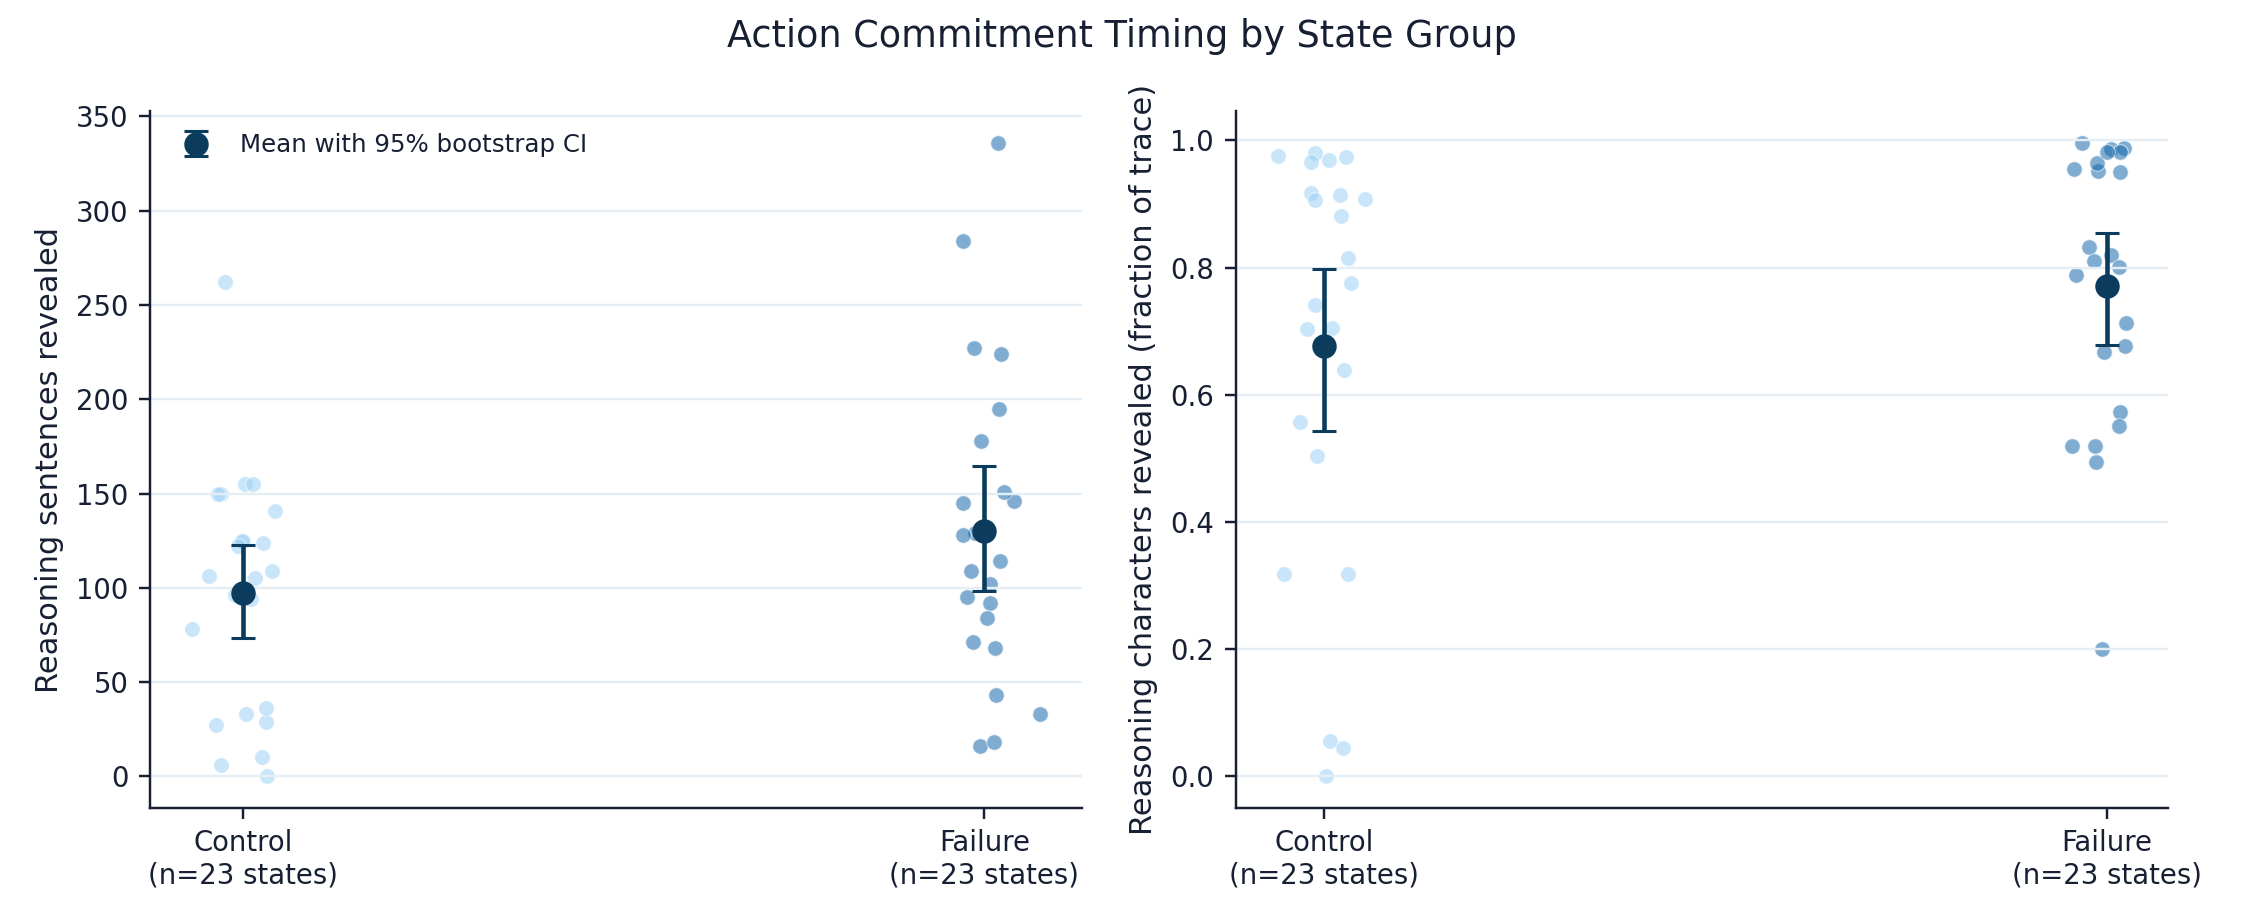
\includegraphics[width=\columnwidth]{figures/commitment_timing_matched46.png}
\caption{Commitment timing in 46 matched decisions. The left panel reports the
sentence index at commitment; the right reports the fraction of reasoning
characters revealed. Points are decisions. Large markers are group means and
bars are 95\% intervals obtained by resampling decisions within each group.}
\label{fig:commitment-timing-matched46}
\end{figure}

\paragraph{Belief-clause sufficiency control.}
For 46 decisions from 31 trajectories, we remove the chain of thought while
retaining the grid and key status, then add one fixed block of clauses. Actions
are obtained from candidate-token probabilities at temperature $0.7$.

\begin{table}[htbp]
\centering
\small
\begin{tabular}{lrrr}
\toprule
Condition & Different & Mean TV & Optimal \\
\midrule
Full CoT & 0/46 & 0.000 & 38/46 \\
Grid only & 34/46 & 0.723 & 17/46 \\
Model reports & 31/46 & 0.677 & 23/46 \\
Verified facts & 36/46 & 0.767 & 11/46 \\
One false wall fact & 36/46 & 0.750 & 20/46 \\
Irrelevant clauses & 31/46 & 0.686 & 22/46 \\
\bottomrule
\end{tabular}
\caption{Action readouts after replacing the chain of thought with state-belief
clauses. ``Different'' counts decisions whose top action differs from the
full-chain action. TV is total variation distance from the full-chain action
distribution. Verified facts are simulator-derived; the false condition flips
one wall fact.}
\label{tab:belief-clause-sufficiency}
\end{table}

The model-report and irrelevant-clause conditions differ little in optimal
rate, while verified facts perform worse than either. The six local facts are
therefore not a sufficient replacement for the chain of thought. The
irrelevant-clause result also shows that wording and clause order remain
confounds.

\paragraph{Offline action-distribution change points.}
A trend-only BEAST analysis detects 160 change points across 44 of 46 decisions.
Of these, 86.9\% lie within three sentences of a recommendation change, compared
with 65.3\% for progress-matched control sentences (randomisation
$p=0.0005$). Proximity is also above the matched rate for optimality losses
(33.1\% versus 26.2\%, $p=0.0060$) and recoveries (41.9\% versus 29.4\%,
$p=0.0005$). Detection uses the complete action-probability series, so these
are retrospective candidate boundaries rather than online predictions or
causal events.

\paragraph{Semantic labels at change points.}
We compare 160 detected change-point sentences with 160 blinded, same-decision
controls matched on reasoning progress and sentence length. The primary test
uses the 152 pairs within $0.10$ reasoning progress. The four-way semantic
distributions do not differ reliably (paired permutation $p=0.219$). Route
deliberation is 5.3 percentage points more frequent at change points, but its
95\% interval obtained by resampling complete trajectories,
$[-2.1,12.0]$, includes zero. These
results do not support a single verbal operation underlying action changes.

\paragraph{Activation event classification.}
Across 7,038 sentence positions from 46 decisions, layer-15 sentence-mean
activations are associated with contemporaneous action-change labels (linear
CKA $0.00437$, permutation-null mean $0.00062$, $p=0.005$). Adding belief
and activation features to a behavioural baseline improves action-change
AUROC by $0.030$ and log loss by $0.0085$ on complete trajectories excluded
from fitting. For
optimal-to-suboptimal transitions, however, the best added signal is the belief
panel and it does not improve held-out performance (AUROC change $-0.011$,
log-loss improvement $-0.0009$). Association at an event is therefore not
evidence of advance prediction or causal use.

\subsection{Judge-generated Semantic Labels}
\label{app:judge_semantic_labels}

\paragraph{Data and annotation.}
This analysis covers 7,038 sentences from 46 matched decisions in 31
trajectories. It uses different data and labels from the four-class analysis of
141,377 sentences from 1,004 decisions in \Cref{sec:reasoning}; the 20,366
sentences used to interpret the activation clusters are a subset of that larger
analysis. The present data come from the same matched cohort as the
reasoning-time action, belief, and activation analyses, although their exact
rows differ after alignment and filtering.

A \texttt{gpt-oss-20b} judge receives the preceding reasoning
and target sentence, with later reasoning and experimental measurements hidden.
It may assign more than one of nine functions: state readout, route planning,
verification, correction, new inference, consolidation, restatement,
procedural continuation, and action commitment. We ran the same prompt twice
independently. Both runs produced valid labels for 7,036 sentences. Exact label
sets agree on 74.9\% of sentences, with an interval of
$[73.8\%,75.9\%]$ from resampling complete trajectories. Derived primary
labels agree on 85.4\% with an interval of $[84.4\%,86.5\%]$ and Cohen's
$\kappa=0.820$. These values measure annotation
repeatability, not agreement with human labels.

\begin{table}[htbp]
\centering
\small
\begin{tabular}{lrr}
\toprule
Function & Run 1 rate & Between-run Dice \\
\midrule
State readout & 36.9\% & 0.923 \\
Route planning & 21.4\% & 0.918 \\
Verification & 21.5\% & 0.823 \\
Correction & 0.4\% & 0.632 \\
New inference & 39.7\% & 0.872 \\
Consolidation & 1.4\% & 0.558 \\
Restatement & 11.5\% & 0.777 \\
Procedural continuation & 5.1\% & 0.915 \\
Action commitment & 5.6\% & 0.934 \\
\bottomrule
\end{tabular}
\caption{Frequency and repeatability of the matched-cohort semantic labels.
Rates need not sum to 100\% because labels may overlap. Dice measures agreement
on the positive examples for each label across two independent runs.}
\label{tab:semantic-label-repeatability}
\end{table}

\paragraph{Temporal structure and prediction.}
The labels occur in a reproducible order. Relative to labels shuffled within
each trajectory and reasoning-progress bin, adjacent primary labels contain
0.118 and 0.120 additional bits of mutual information in the two runs
($p=0.0002$ for each). Twelve
label-to-label transitions and 27 three-sentence sequences are enriched after
false-discovery-rate correction in both runs. However, adding the current
semantic labels to action probabilities, action entropy, reasoning progress,
regime duration, and regime history does not improve prediction of later
regime changes in any of 28 corrected horizon tests. The labels describe
recurring reasoning sequences but do not provide an additional action-change
monitor in this dataset.



\subsection{Answer Forcing}
\label{app:answer-forcing}
For the prefix-level action distributions of \Cref{sec:commitment} (98,310 prefixes), we truncate the reasoning trace at the prefix and append a fixed 12-token suffix that closes the reasoning channel and opens the final-answer JSON in the model's chat format:
\begin{quote}
\ttfamily
<|end|><|start|>assistant<|channel|>final<|message|>\{\par
\ \ "action": "
\end{quote}
The token sequence of the suffix is checked against the tokenizer at load time.
We read the logits of the four single-token candidates \texttt{UP}, \texttt{DOWN}, \texttt{LEFT}, and \texttt{RIGHT} at the next position and normalise them with a softmax; no natural-language instruction is added, and every prefix is scored with an independent forward pass without reuse of cached model state.

\subsection{Action-Mention Classification}
\label{app:action-mentions}
The pre-verbal control and the first-mention timing measure require the position of the first \emph{decisional} mention of an action in each reasoning trace.
We locate every occurrence of \textsc{up}, \textsc{down}, \textsc{left}, or \textsc{right} in the 1,276 traces (72,561 occurrences) at its token position and classify it with fixed rules applied in order: (i) \emph{idiom} --- ``pick up'', ``set up'', ``what's left'', ``that's right'' and similar (0.9\%); (ii) \emph{negated} --- a negation cue within two words before the word (``cannot go up'', ``instead of right'') or ``is blocked'', ``is a wall'', ``is not possible'' within three words after it (3.3\%); (iii) \emph{answer} --- preceded by ``answer'', ``action'', ``output'', ``choose'' or similar (3.0\%); (iv) \emph{movement} --- preceded by a movement verb such as ``go'', ``move'', ``head'', ``step'' (18.3\%); (v) \emph{capitalised} direction words (6.4\%); (vi) \emph{descriptive} --- preceded by ``to/on/at the'', ``top-'', ``bottom-'', or followed by ``side'', ``column'', ``of'', ``wall'', ``corner'' and similar (5.8\%); (vii) \emph{bare} --- all remaining occurrences, mostly route enumerations such as ``left to (1,6), left to (1,5)'' (62.2\%).
Classes (iii)--(v) and (vii) are decisional; (i), (ii) and (vi) are not.
Under the previous definition (any direction word, regardless of context) the pre-verbal subset contained 31,723 prefixes and the median first mention was at progress 0.25; under the decisional definition it contains 35,379 prefixes and the median first decisional mention is at 0.30, with 37.0\% of decisions committing before it (35.6\% under the previous definition).
Counting negated mentions as decisional changes the subset by 46 prefixes and none of the reported values.


\subsection{Reasoning-Step Clustering Details}
\label{app:reasoning-clustering}

This appendix provides additional details on the sentence-level activation
clustering used in \Cref{sec:reasoning-patterns}. The main analysis uses
sentence-mean representations from layer 15 of \texttt{gpt-oss-20b}. For
each reasoning sentence, we mean-pool the token-level hidden states over the
sentence span to obtain one 2,880-dimensional vector. We randomly sample
25,000 of the 153,622 sentence representations, reduce them to 100 principal
components retaining 77.84\% of the activation variance, and
$\ell_2$-normalise the resulting vectors before clustering.

\paragraph{Clustering method comparison.}
We compare MiniBatch K-means, HDBSCAN, and Gaussian mixture models using both
sentence-mean and sentence-final representations. Sentence-mean HDBSCAN
achieves the highest silhouette coefficient and lowest intra-cluster
dispersion, but assigns 77.1\% of sentences to noise. Sentence-mean K-means
provides a complete partition of the data and achieves the highest
inter-cluster dispersion and Calinski--Harabasz score among the
complete-coverage methods. We therefore use sentence-mean K-means for the
main analysis, while treating HDBSCAN as a secondary method for identifying
high-density motifs.

\td{Specify how the number of K-means clusters, $K=12$, was selected.}

\begin{table}[htbp]
\centering
\small
\begin{tabular}{lccccc}
\toprule
Method & Silhouette & Inter-disp. & Intra-disp. & CH & Noise \\
\midrule
Mean K-means     & 0.138 & 905.0 & 0.600 & 1509.0 & 0.0\% \\
Mean HDBSCAN     & 0.431 & 263.9 & 0.225 & 1172.9 & 77.1\% \\
Mean GMM         & 0.075 & 755.6 & 0.666 & 1135.3 & 0.0\% \\
Final K-means    & 0.128 & 782.6 & 0.655 & 1194.0 & 0.0\% \\
Final HDBSCAN    & 0.381 & 297.2 & 0.293 & 1014.0 & 64.8\% \\
Final GMM        & 0.074 & 641.3 & 0.718 & 893.7 & 0.0\% \\
\bottomrule
\end{tabular}
\caption{Clustering quality for sentence-mean and sentence-final hidden
representations. Inter-dispersion and intra-dispersion measure separation
between clusters and compactness within clusters, respectively. CH denotes
the Calinski--Harabasz score.}
\label{tab:reasoning-clustering}
\end{table}

\begin{figure}[htbp]
    \centering

    \begin{subfigure}[t]{0.49\textwidth}
        \centering
        \includegraphics[width=\linewidth]{figures/hdbscan_mean.png}
        \caption{HDBSCAN}
        \label{fig:hdbscan-clusters}
    \end{subfigure}
    \hfill
    \begin{subfigure}[t]{0.49\textwidth}
        \centering
        \includegraphics[width=\linewidth]{figures/k_means_mean.png}
        \caption{MiniBatch K-means}
        \label{fig:kmeans-clusters}
    \end{subfigure}

    \caption{
    Two-dimensional PCA visualisation of sentence-level hidden
    representations. HDBSCAN identifies a smaller number of dense regions
    while assigning many points to noise, whereas K-means provides a complete
    partition of the representation space.
    }
    \label{fig:clustering-comparison}
\end{figure}

\paragraph{Cluster interpretation.}
The clustering procedure is unsupervised and does not use semantic labels.
For interpretation only, we inspect representative sentences from each
cluster and compare cluster assignments with independently assigned semantic
reasoning annotations. We then attach short descriptive names to the numeric
cluster IDs. These names are post-hoc summaries and are not used during
clustering.

Among 20,366 sentences with exact alignment to the semantic annotations,
K-means reaches normalised mutual information of 0.131. Thus, the activation
clusters capture structure that is related to, but not identical with, the
semantic categories. HDBSCAN yields higher semantic purity on its non-noise
subset, with normalised mutual information of 0.297 and homogeneity of
0.473, but leaves approximately 80\% of downstream sentences unassigned.

\begin{table}[htbp]
\centering
\small
\begin{tabular}{lll}
\toprule
Cluster & Descriptive interpretation & Example reasoning role \\
\midrule
\(C_0\)  & Path initiation & Beginning or extending a route \\
\(C_1\)  & Local world-state checking & Reading nearby grid structure \\
\(C_2\)  & Route execution & Following a selected path \\
\(C_3\)  & Door-mechanics reasoning & Reasoning about key or door state \\
\(C_4\)  & Alternative-route exploration & Considering another route \\
\(C_5\)  & Grid-state setup & Reconstructing the current state \\
\(C_6\)  & Detailed state readout & Explicitly checking environment details \\
\(C_7\)  & Route consolidation & Consolidating a planned path \\
\(C_8\)  & Blockage verification & Checking whether a movement is blocked \\
\(C_9\)  & Local route tracing & Tracing immediate movement options \\
\(C_{10}\) & Decision revision & Revising or transitioning between choices \\
\(C_{11}\) & Action conclusion & Expressing or consolidating the final action \\
\bottomrule
\end{tabular}
\caption{Post-hoc descriptive interpretations of the K-means clusters.
Cluster IDs are used throughout the quantitative analysis; the descriptions
are provided only to aid interpretation.}
\label{tab:cluster-labels}
\end{table}

\td{Add one or two representative sentences for each cluster, ideally in a
separate table or supplementary file.}

The coarse semantic comparison is consistent with several of these
descriptions. Clusters \(C_6\), \(C_5\), and \(C_1\) contain a larger
proportion of world-reading sentences, whereas \(C_2\), \(C_7\), and \(C_4\)
contain more solving-oriented sentences. \(C_{11}\) contains a larger
answering component. A finer multi-label analysis also shows enrichment for
specific reasoning functions: \(C_2\) is enriched approximately
\(9.8\times\) for action commitment, \(C_{10}\) \(10.1\times\) for
correction, \(C_8\) \(2.8\times\) for verification, and \(C_0\)
\(5.6\times\) for procedural continuation.

\paragraph{Cluster frequencies around commitment.}
The distribution of clusters changes across the commitment point. After
commitment, \(C_{11}\), \(C_2\), and \(C_7\) increase in frequency by
12.8, 6.3, and 5.6 percentage points, respectively. In contrast, \(C_5\),
\(C_6\), \(C_0\), and \(C_1\) decrease by 9.8, 7.4, 4.4, and 2.7 percentage
points. This pattern is consistent with a transition from state
interpretation and revision toward route execution and explicit action
conclusion.

To control for the fact that commitment tends to occur at particular
positions in the reasoning trace, we compare true commitment sentences with
position-matched control sentences drawn from the same decisions. The largest
difference is observed for \(C_{10}\), which occurs in 14.0\% of true
commitment sentences compared with 5.9\% under the matched control. Smaller
excesses are observed for \(C_9\) and \(C_2\).

\begin{table}[htbp]
\centering
\small
\begin{tabular}{lrrr}
\toprule
Cluster & True commitment & Matched control & Excess \\
\midrule
\(C_{10}\) & 14.0\% & 5.9\% & \(+8.2\) pp \\
\(C_9\)    & 11.6\% & 8.4\% & \(+3.2\) pp \\
\(C_2\)    & 9.3\% & 6.8\% & \(+2.5\) pp \\
\(C_5\)    & 15.1\% & 13.5\% & \(+1.6\) pp \\
\(C_7\)    & 5.5\% & 4.5\% & \(+1.0\) pp \\
\bottomrule
\end{tabular}
\caption{Frequency of selected K-means clusters at true commitment positions
and at position-matched control positions from the same decisions.}
\label{tab:commitment-clusters-app}
\end{table}

\td{Add uncertainty estimates or statistical tests for the commitment versus
matched-control comparison.}

\paragraph{Clusters at action-revision events.}
We also test whether particular activation-defined reasoning states are
associated with changes in the currently preferred action. Approximately
4.59\% of reasoning sentences contain at least one such change. Relative to
a within-decision shuffled-event control, \(C_6\), \(C_{10}\), \(C_9\), and
\(C_5\) are enriched at action-preference changes by factors of
\(1.65\times\), \(1.64\times\), \(1.41\times\), and \(1.33\times\),
respectively. All four effects remain significant after false-discovery-rate
correction (\(q=0.0024\)) \cite{benjamini1995controlling}.

The same clusters occur around both losses and recoveries of action
optimality. For optimal-to-suboptimal transitions, enrichment factors are
\(2.07\times\), \(1.48\times\), \(1.45\times\), and \(1.26\times\) for
\(C_6\), \(C_{10}\), \(C_9\), and \(C_5\), respectively. For
suboptimal-to-optimal transitions, the corresponding factors are
\(1.77\times\), \(1.59\times\), \(1.44\times\), and \(1.35\times\).
Because the same clusters are associated with both directions of change, we
interpret them as reasoning states associated with decision revision rather
than as error-specific states.

\begin{table}[htbp]
\centering
\small
\begin{tabular}{lccc}
\toprule
Cluster & Action change & Accuracy drop & Accuracy recovery \\
\midrule
\(C_6\)    & \(1.65\times\) & \(2.07\times\) & \(1.77\times\) \\
\(C_{10}\) & \(1.64\times\) & \(1.48\times\) & \(1.59\times\) \\
\(C_9\)    & \(1.41\times\) & \(1.45\times\) & \(1.44\times\) \\
\(C_5\)    & \(1.33\times\) & \(1.26\times\) & \(1.35\times\) \\
\bottomrule
\end{tabular}
\caption{Enrichment of sentence-level activation clusters at
action-preference changes and changes in action optimality, relative to
within-decision shuffled-event controls.}
\label{tab:reasoning-events-app}
\end{table}

The immediately preceding sentence shows a similar pattern. For example,
\(C_5\) is enriched \(2.09\times\) before an optimal-to-suboptimal transition
and \(2.47\times\) before a suboptimal-to-optimal transition.

\paragraph{Exploratory cluster sequences.}
Finally, we examine whether short transitions between activation clusters are
overrepresented near commitment. Examples include
\(C_8\!\rightarrow C_{10}\) (\(4.75\times\)),
\(C_{10}\!\rightarrow C_{10}\) (\(2.87\times\)), and
\(C_7\!\rightarrow C_{10}\) (\(2.71\times\)). Enriched three-step sequences
include \(C_6\!\rightarrow C_5\!\rightarrow C_5\) (\(3.26\times\)) and
\(C_{10}\!\rightarrow C_{10}\!\rightarrow C_{10}\) (\(3.86\times\)).
Because the number of possible sequences is large and these analyses are
exploratory, we do not use them to support the main conclusions.
%%%%%%%%%%%%%%%%%%%%%%%%%%%%%%%%%%%%%%%%%%%%%%%%%%%%%%%%%%%%

\newpage
\input{checklist.tex}


\end{document}